\documentclass{workbook}

\newcommand{\copyrightdate}{2025}

\usepackage{ifxetex}
\usepackage[utf8]{inputenc}
\usepackage{hyperref}
\usepackage{hyperxmp} % Embed meta data into the PDF
\hypersetup{%
	hidelinks=true,
	linkcolor = {0 0 1},
	% Metadata to be embedded by hyperxmp
	pdftitle={Calculus II (\jobname)},
	pdfauthor={Jason Siefken, Geoff McGregor, Arman Pannu},
	pdfauthortitle={Author},
	pdfcopyright={Copyright (C) \copyrightdate, Jason Siefken, Geoff McGregor, Arman Pannu},
	pdfsubject={Calculus 2 textbook/workbook},
	pdfkeywords={calculus 2},
	pdfurl={https://github.com/siefkenj/MAT187-2025/},
	pdflicenseurl={https://creativecommons.org/licenses/by-sa/4.0/},
}

%%%
% import all needed packages and macros
%%%
\usepackage[yyyymmdd]{datetime}
\input{common/preamble.tex}

\usepackage{breqn}

\usepackage{pdfrender} % For text title


%%%
% Set up the footers to have the correct copyright notices
%%%

\fancypagestyle{siefken}{%
	\rfoot{\footnotesize\it \copyright\,Geoff McGregor, Arman Pannu \& Jason Siefken, \copyrightdate \ \makebox(30,5){\includegraphics[height=1.2em]{by-sa.pdf}}}
	\lfoot{}
	\renewcommand{\headrulewidth}{0pt}
}


%%
% Allow hiding of environments
%%
\usepackage{environ}% http://ctan.org/pkg/environ
\makeatletter
\newcommand{\voidenvironment}[1]{%
  \expandafter\providecommand\csname env@#1@save@env\endcsname{}%
  \expandafter\providecommand\csname env@#1@process\endcsname{}%
  \@ifundefined{#1}{}{\RenewEnviron{#1}{}}%
}
\makeatother
% allow pagebreaks that only display in `standard` mode
\newcommand{\displayonlynewpage}{\begin{displayonly}\newpage\end{displayonly}}
% allow pagebreaks that only display in `book` mode
\newcommand{\bookonlynewpage}{\begin{bookonly}\newpage\end{bookonly}}


%
% Set up the three render modes: standard, instructor, and solutions.
% These render with varying amounts of extra data (like solutions and notes)
%
\newtoggle{instructor}
\newtoggle{standard}
\newtoggle{solutions}
\newtoggle{book}
\newtoggle{slides}
\newtoggle{slideswhite}
\newcommand{\setinstructor}{
	\toggletrue{instructor}
	\togglefalse{standard}
	\togglefalse{solutions}
	\togglefalse{book}
	\togglefalse{slides}
	\togglefalse{slideswhite}
}
\newcommand{\setstandard}{
	\togglefalse{instructor}
	\toggletrue{standard}
	\togglefalse{solutions}
	\togglefalse{book}
	\togglefalse{slides}
	\togglefalse{slideswhite}
}
\newcommand{\setsolutions}{
	\togglefalse{instructor}
	\togglefalse{standard}
	\toggletrue{solutions}
	\togglefalse{book}
	\togglefalse{slides}
	\togglefalse{slideswhite}
}
\newcommand{\setbook}{
	\togglefalse{instructor}
	\togglefalse{standard}
	\togglefalse{solutions}
	\toggletrue{book}
	\togglefalse{slides}
	\togglefalse{slideswhite}
}
\newcommand{\setslides}{
	\togglefalse{instructor}
	\togglefalse{standard}
	\togglefalse{solutions}
	\togglefalse{book}
	\toggletrue{slides}
	\togglefalse{slideswhite}
}
\newcommand{\setslideswhite}{
	\togglefalse{instructor}
	\togglefalse{standard}
	\togglefalse{solutions}
	\togglefalse{book}
	\togglefalse{slides}
	\toggletrue{slideswhite}
}


%
% Infer the document level from the \jobname
%
\usepackage{xstring}
\IfSubStr{\jobname}{\detokenize{book}}{\setbook}{
	\IfSubStr{\jobname}{\detokenize{solutions}}{\setsolutions}{
		\IfSubStr{\jobname}{\detokenize{instructor}}{\setinstructor}{
			\IfSubStr{\jobname}{\detokenize{slides}}{\setslides}{
				\IfSubStr{\jobname}{\detokenize{white}}{\setslideswhite}{
						\setstandard
				}
			}
		}
	}
}


\setbookoptions{
	twosided = false,
	inline solutions = false,
}


\NewColoredEnvironment{
	name = lesson,
	display name = Lesson,
	banner color = Plum,
	title color = Plum,
	banner on left = true,
	open right = false,
}
\NewColoredEnvironment{
	name = module,
	display name = Module,
	banner color = Turquoise,
	title color = Cerulean,
	definition color = Cerulean,
	theorem color = myorange,
}
\NewColoredEnvironment{
	name = appendix,
	display name = Appendix,
	banner color = LimeGreen,
	title color = LimeGreen!70!Green!80!black,
	definition color = Cerulean,
	theorem color = myorange,
}
\NewColoredEnvironment{
	name = indices,
	display name = Indices,
	banner color = Green,
	title color = Green,
}
\NewColoredEnvironment{
	name = tutorial,
	display name = Tutorial,
	banner color = Peach,
	title color = Peach!80!black,
	emphbox color = Peach,
	% We will print tutorial worksheets back-to-back to save space
	open right = false,
}




\loadgeometry{default}

%
% Hide the non-problem environments
%
\newcommand{\coversubtitle}{} % we override the subtitle in each mode, so make sure the command exists to override.
\iftoggle{instructor}{
	\voidenvironment{module}
	\voidenvironment{appendix}
	\voidenvironment{bookonly}
	\voidenvironment{displayonly}
	\renewcommand{\coversubtitle}{Instructor Guide}
}{}
\iftoggle{solutions}{
	\voidenvironment{module}
	\voidenvironment{appendix}
	\voidenvironment{bookonly}
	\voidenvironment{displayonly}
	\voidenvironment{lesson}
	\voidenvironment{notes}
	\renewcommand{\coversubtitle}{Solutions}
}{}
\iftoggle{standard}{
	\voidenvironment{module}
	\voidenvironment{appendix}
	\voidenvironment{bookonly}
	\voidenvironment{solution}
	\voidenvironment{annotation}
	\voidenvironment{lesson}
	\renewcommand{\coversubtitle}{MAT187 Notes}
	\loadgeometry{default}
}{}
\iftoggle{book}{
	\voidenvironment{displayonly}
	\voidenvironment{solution}
	\voidenvironment{annotation}
	\voidenvironment{lesson}
	\renewcommand{\coversubtitle}{{\hspace{-5pt}\begin{tabular}{l}MAT187 Workbook\\\small\today{} Edition\end{tabular}}}
	\setbookoptions{
		twosided = true,
		inline solutions = false,
	}
	\loadgeometry{book}
}{}
\iftoggle{slides}{
	\voidenvironment{module}
	\voidenvironment{appendix}
	\voidenvironment{bookonly}
	\voidenvironment{solution}
	\voidenvironment{annotation}
	\voidenvironment{lesson}
	\renewcommand{\coversubtitle}{MAT187 Slides}
	\loadgeometry{slides}
	\initSlides
}{}
\iftoggle{slideswhite}{
	\voidenvironment{module}
	\voidenvironment{appendix}
	\voidenvironment{bookonly}
	\voidenvironment{solution}
	\voidenvironment{annotation}
	\voidenvironment{lesson}
	\renewcommand{\coversubtitle}{\hspace{-70pt}MAT187 Student Slides}
	\loadgeometry{slides}
	\initSlidesWhite
}{}
%\voidenvironment{solution}
%\voidenvironment{annotation}
%\voidenvironment{lesson}
%%\voidenvironment{notes}
%%\voidenvironment{displayonly}

% Allow an index to be created
\makeindex[title=Index of Terms, columns=3]
\makeindex[name=definitions, title=Index of Definitions, columns=3]
\makeindex[name=symbols, title=Index of Symbols, columns=3]

\indexsetup{
	level=\Heading,
	noclearpage
}

\begin{document}
%%
%% Import definitions from definition.tex; all definitions can be restated multiple times
%%

\input{common/definitions.tex}

%%
%% End Definitions
%%


\definecolor{forestgreen}{rgb}{0.13, 0.55, 0.13}

% Needed to get different PDF bookmarks from the TOC entries
\hypersetup{bookmarksdepth=3}

\pagestyle{empty}

\input{common/cover.tex}

\newpage

\begin{bookonly}
	\clearpage
	\hbox{}
	\newpage
	\input{modules/preface.tex}
	\section*{Contributors}
	\input{common/contributors.tex}
	\section*{Dedication}
	\begin{center}
		This book is dedicated to
		\href{https://www.gazettetimes.com/news/local/obituaries/dr-robert-main-burton/article_9c087f07-c005-515a-bb3f-2c9c6a6b7332.html}{\color{blue}Dr.~Bob Burton}---friend and mentor.

		\emph{\large ``Sometimes you have to walk the mystical path with practical feet.''}
	\end{center}
	\newpage
	\mbox{}
	{
		\pagestyle{empty}
		\setcounter{tocdepth}{1}
		\tableofcontents
		\thispagestyle{empty}
	}
	\newpage
	\mbox{}
	\newpage
\end{bookonly}

\setcounter{page}{1}
\pagestyle{siefken}


\addcontentsline{toc}{chapter}{Lessons}


%
% Hours 1-6
%

\begin{slide}
	\question
	Consider the plot of the complex numbers $p_1$, $p_2$, $p_3$, $p_4$ in the complex plane.

	\includegraphics[width=2.4in]{complex1.jpg}

	\begin{parts}
		\item For which complex numbers is the real part grater than the imaginary part?
		\item Which complex number has the smallest \emph{modulus}/\emph{absolute value}?
		\item Which complex number has the largest \emph{argument}?
		Is your answer at all ambiguous?
	\end{parts}
\end{slide}

\begin{slide}
	\question
	Consider the plot of the complex number $p$ in the complex plane.

	\includegraphics[width=2.4in]{complex2.jpg}

	\begin{parts}
		\item Sketch the complex number $2p$.
		\item Sketch the complex number $p^2$.
		\item Sketch the complex numbers $p^n$ for $n=3,4,\ldots$. Will your answer 
		depend on $r$?

		\bigskip 
		\item Use the geometry of the complex plane to find $\sqrt{i}$. Express
		your answer in both polar and rectangular form.
	\end{parts}
\end{slide}

\begin{slide}
	\question
	Consider the equation 
	\begin{equation}
		\label{eq:complex}
		z^3=-1
	\end{equation}

	\begin{parts}
		\item Find a solution to Equation \eqref{eq:complex}.
		\item If $z=re^{i\theta}$ is a solution to Equation \eqref{eq:complex}, 
		what conditions must $r$ and $\theta$ satisfy? Justify your conclusions.
		\item Find all solutions to Equation \eqref{eq:complex}.

	\end{parts}
\end{slide}

%\begin{slide}
%	\question
%	Consider the equation 
%	\begin{equation}
%		\label{eq:complex2}
%		z^n=1,
%	\end{equation}
%
%    where $n$ is a positive integer.
%
%	\begin{parts}
%		\item Solutions to Equation \eqref{eq:complex2} are called \emph{roots of unity}.
%		How many roots of unity are there (for a fixed value of $n$)?
%		\item Find the roots of unity for $n=4$.
%		\item Let $n=4$. Geometrically, what should the \emph{sum} of the roots of unity be?
%		Verify your answer algebraically.
%		\item Let $n=5$. What should the sum of the roots of unity be? 
%
%	\end{parts}
%\end{slide}

\begin{slide}
	\question
	For each situation, decide whether \emph{least squares} curve fitting
	or \emph{polynomial interpolation} would be more appropriate.

	\begin{parts}
		\item You are modelling the arch used in the construction of a 
		particular Roman aqueduct. You have collected several hundred data points
		of height of the arch vs. distance from the base of the aqueduct.

		\item You are creating a function to govern the brightness of a light
		which will be used for signalling a computer. There are three different brightnesses
		that must be achieved exactly and the transition between those brightnesses must be smooth.

		\item You are given exact data points from a lab and told that the data was created with a 4th 
		degree polynomial. You are asked to find the coefficients of the polynomial.
	\end{parts}
\end{slide}

\begin{slide}
	\question
	A baseball is thrown on the moon. You are trying to find the function
	\begin{itemize}
		\item $h(t)$, the height (in meters)of the baseball above the moon's surface at time $t$ (in seconds).
	\end{itemize}
	You collected the following data

	% Comes from the equation -.8t^2+2.2t+2.6
	\begin{center}
	\begin{tabular}{|c|c|}
		\hline
		$t$ & $h(t)$\\
		\hline
		1 & 4\\
		2 & 3.8\\
		3 & 2\\
		\hline
	\end{tabular}
	\end{center}

	\begin{parts}
		\item What degree polynomial would best model $h$?
		\item Use polynomial interpolation to find $h$.
		\item Find the maximum height of the baseball above the moon's surface.
		\item What would change (if anything) if you were given 4 data points?
	\end{parts}
\end{slide}

\begin{slide}
	\question
		While developing a robotics control system, you find the need for
		a function $f$ which satisfies the following properties:
	\begin{enumerate}
		\item[(i)] $f(0)=-1$ and $f(1)=2$
		\item[(ii)] $f'(0)=-1$ and $f'(1)=2$
	\end{enumerate}
	Your friend suggests that you could use the following polynomial to come up with $f$:
	\[
		L_1(x)=-(x-1) \qquad\phantom{x}\qquad L_2(x)=x
	\]
	\[
		S_1(x)=(x-1)^2x \qquad S_2(x)=(x-1)x^2
	\]

	\begin{parts}
		\item Can Lagrange interpolation be used to directly find $f$? Explain.
		\item Complete the following table
		\begin{center}
		\begin{tabular}{|c|c|c|c|c|}
			\hline
			$g$ & $g(0)$ & $g(1)$ & $g'(0)$ & $g'(1)$\\
			\hline
			$L_1$ & & & & \\
			\hline
			$L_2$ & & & & \\
			\hline
			$S_1$ & & & & \\
			\hline
			$S_2$ & & & & \\
			\hline
		\end{tabular}
		\end{center}
		\item Use $L_1$, $L_2$, $S_1$, and $S_2$ to find a polynomial satisfying the properties of $f$.
		\item Explain how Lagrange interpolation can be generalized to allow finding a polynomial
		that passes through particular points and takes on particular derivatives at those points.
	\end{parts}
\end{slide}

\begin{slide}
	\question
	\begin{parts}
	\item For each polynomial approximation of the bell curve, is the approximation best at
	$0$, best on the interval $[-2,2]$, or best on the interval $[0,2]$.

	% https://www.desmos.com/calculator/qjruzy8gvw
	(A)~\includegraphics[width=1.25in]{B2-Plot1.png}
	(B)~\includegraphics[width=1.25in]{B2-Plot2.png}\\
	(C)~\includegraphics[width=1.25in]{B2-Plot3.png}
	(D)~\includegraphics[width=1.25in]{B2-Plot4.png}
	% Show list of 4 pictures approximating (a bell curve?) with 
	% different styles of approximation
	\item Based on the pictures, which polynomial(s) do you think come from a Taylor approximation?
	\end{parts}
\end{slide}

\begin{slide}
	\question
	The function $f$ satisfies
	\[f(0)= 1\qquad f'(0)=0\qquad f''(0)=-2\]\[ f'''(0)=0\qquad f''''(0)=12\]

	\begin{parts}
		\item Write down $T_4$, the 4th degree Taylor approximation to $f$ centered at $0$.
		\item Use Desmos to compare the graph of $T_4$ with the graphs of $g_1$,
		$g_2$, $g_3$, and $g_4$. Which of the $g$'s do you think is most likely equal to $f$?
		\begin{enumerate}
			\item $g_1(x)=e^{-|x|}$
			\item $g_2(x)=e^{-x^2}$
			\item $\displaystyle g_3(x)=\frac{1}{1+x^2}$
			\item $\displaystyle g_4(x)=\frac{1}{1+(2x)^4}$
		\end{enumerate}
	\end{parts}

	% list equations of previous 4 approximations
\end{slide}



\begin{slide}
	\question
	A bee is flying back and forth along a window sill trying to escape from your living room. 

	The bee's position at time $t$ along the window sill is given by $r(t)$.

	You know that a first-order Taylor approximation to $r(t)$ at time $t=2$
	is
	\[
		A_1(t)=3(t-2)+1
	\]

	\begin{parts}
		\item Estimate the position of the bee on the window sill at time 
		$2.1$. Is your answer exact or approximate?
		\item Estimate the velocity of the bee at time $2.1$. Is your answer exact or approximate?
		\item Are there any times you can compute the \emph{exact} position of the bee?
		\item Are there any times you can compute the \emph{exact} velocity?
		\item What is your best estimate for the acceleration of the 
		bee at time $2.1$?
	\end{parts}
\end{slide}

\begin{slide}
	\question
	A bee is flying back and forth along a window sill trying to escape from your living room. 

	The bee's position at time $t$ along the window sill is given by $r(t)$.
	
	You know that a second-order Taylor approximation to $r(t)$ at time $t=2$
	is
	\[
		A_2(t)=2(t-2)^2 + 3(t-2) + 1
	\]

	\begin{parts}
	\item Estimate the position of the bee on the window sill at time 
		$2.1$. Is your answer exact or approximate?
		\item Estimate the velocity of the bee at time $2.1$. Is your answer exact or approximate?
		\item Are there any times you can compute the \emph{exact} position of the bee?
		\item Are there any times you can compute the \emph{exact} velocity?
		\item What is your best estimate for the acceleration of the 
		bee at time $2.1$?
	\end{parts}
\end{slide}

\begin{slide}
	\question
	Based on the pictures, which polynomial approximations of the bell curve do you think
	are \emph{Taylor} polynomials?

	(A)~\includegraphics[width=1.25in]{B2-Plot1.png}
	(B)~\includegraphics[width=1.25in]{B2-Plot2.png}\\
	(C)~\includegraphics[width=1.25in]{B2-Plot3.png}
	(D)~\includegraphics[width=1.25in]{B2-Plot4.png}
	% Show list of 4 pictures approximating (a bell curve?) with 
	% different styles of approximation
\end{slide}


\begin{slide}
	\question
	Let $f(x)=e^x$ and let $P_n(x)$ be the $n$th Taylor approximation to $f$ centered at $0$. In particular
	\[
		P_3(x)=1+x+\frac{x^2}{2}+\frac{x^3}{6}
	\]
	Let $R_n(x)$ be the (signed) error in $P_n(x)$.

	\begin{parts}
		\item Find $R_3(1.5)$ (you may use a calculator).
		\item What is the largest value of $R_3(x)$ when $0\leq x\leq 2$?
		\item Is there a value of $x$ for which $R_3(x)=0$? What does this 
		say about $P_3$?

		\medskip 
		\item Given that $|f^{(5)}(x)| \leq 8$ when $x\in [0,2]$, 
		find an upper bound for $R_4(x)$ that
		\begin{enumerate}
			\item works for a fixed $x\in[0,2]$
			\item works simultaneously for all $x\in[0,2]$
		\end{enumerate}
		\item Given what you know from the previous part(s), can you bound $R_n(x)$?
	\end{parts}
\end{slide}


\begin{slide}
	\question
	Let $f$ be an infinitely differentiable function, and let $P_n$ be a
	a Taylor polynomial for $f$ of degree $n$ centered at $a$.

	We approximate $f(x)\approx P_n(x)$. Which of the following affect the
	size of the error in $P_n(x)$ (i.e., the magnitude of $R_n(x)$)?

	\begin{enumerate}
		\item[(A)] The degree of $P_n$, i.e., $n$.
		\item[(B)] The magnitude of $f(a)$, i.e., $|f(a)|$.
		\item[(C)] The magnitudes of the derivatives of $f$ at $a$, i.e., the size of $|f'(a)|$, $|f''(a)|$, etc..
		\item[(D)] The distance from $a$ that you are approximating at, i.e., 
		the size of $|x-a|$.

	\end{enumerate}
\end{slide}

\begin{slide}
	\question
	Use Desmos to conjecture about the following questions.

	\url{https://www.desmos.com/calculator/nrru5n0gqq}

	\begin{parts}
		\item True/False? When approximating $\sin(x)$ using Taylor polynomials centered at $x=0$, higher degree polynomials will approximate $\sin(2)$ better.
		\item True/False? When approximating $\tan(x)$ using Taylor polynomials centered at $x=0$, higher degree polynomials will approximate $\tan(2)$ better.

		\item True/False? When approximating $f(x)=\frac{1}{1+x^2}$ using Taylor polynomials centered at $x=0$, higher degree polynomials will approximate $f(2)$ better.

		\item Make a conjecture about the relationship between the degree of your Taylor approximation and the accuracy of its values. Does
		this contradict what you know from Taylor's remainder theorem?

	\end{parts}
\end{slide}


%
% Numerical Integration
%
\begin{slide}
	\question
	Consider the function $f(x)=\frac{1}{2}x^2+1$ and the value $\displaystyle I=\int_{0}^3f(x)\,\mathrm d x$.

	\begin{parts}
		\item Make three sketches: one where the left-endpoint rule is used to approximate $I$, 
		one where the right-endpoint rule is used, 
		and one where the trapezoid rule is used. (Use at least three intervals.)

		\item For the left-endpoint, right-endpoint, and trapezoid rules, which will give over estimates of
		$I$ and which will give underestimates? Will any give an exact value?

		\medskip
		\item Consider the following estimates of $I$:
		\begin{itemize}
			\item $E_1=8.6875$
			\item $E_2=6.4375$
			\item $E_3=7.5625$
		\end{itemize}
		Each estimate comes from using the same partition.

		Which estimates come from a left-endpoint approximation, a right-endpoint approximation, 
		and a trapezoid approximation?

		\emph{Hint: you know calculus!}

		\item (Homework) Will the midpoint rule produce an over or under estimate of $I$?

	\end{parts}
\end{slide}

\begin{slide}
	% https://www.desmos.com/calculator/5lszweq0bd
	\question
	In a classic problem, you are trying to find the volume of a wine barrel. 
	Let $r(\ell)$ represent the radius of the barrel $\ell$ cm from the base. The total
	length of the barrel is 80cm.

	You know the volume of the barrel can be computed exactly by
	\[
		\int_0^{80}\pi [r(\ell)]^2\,\mathrm d \ell.
	\]

	You have measured the barrel in several places and gotten the following data
	\begin{center}
		\begin{tabular}{ccccc}
			r(0)&r(20)&r(40)&r(60)&r(80)\\
			12.8 & 21.2 & 22.7 & 21.4 & 13.4  \\
		\end{tabular}
	\end{center}

	\begin{parts}
		\item Make a sketch of the barrel's profile. Make a second sketch of $\pi [r(\ell)]^2$.

		\item Based on your sketch, do you think using a trapezoid approximation will produce an over 
		or under estimate for the volume?

		\item Use a trapezoid approximation to estimate the volume of the barrel.

		\item Use a Simpson's approximation to estimate the volume of the barrel. 
		
		\emph{Reminder:}
		if $p$ is a quadratic polynomial, 
		\[
		 \int_a^b p(x)\,\mathrm d x = \frac{b-a}{6}\left(p(a)+4p\Big(\frac{a+b}{2}\Big)+p(b)\right)
		 \]

		 \item The exact (rounded) volume of the barrel is 104384cm$^3$. What approximation
		 method was most accurate? Why?


	\end{parts}
\end{slide}

\begin{slide}
	\question
	For this question, the domain of integration will be $0$ to $5$ and you will
	be using a uniform partition with $5$ pieces.

	\begin{parts}
		\item Draw a function where the left endpoint approximation is an \emph{under estimate}.
		
		\item Draw a function where the right endpoint approximation is an \emph{under estimate}.
		
		\item Draw a function where the trapezoid approximation is an \emph{under estimate}.
		
		\item Draw a function where the midpoint approximation is an \emph{under estimate}.

	\end{parts}
\end{slide}


\begin{slide}
	% https://www.desmos.com/calculator/nxyvpewqxs
	\question

	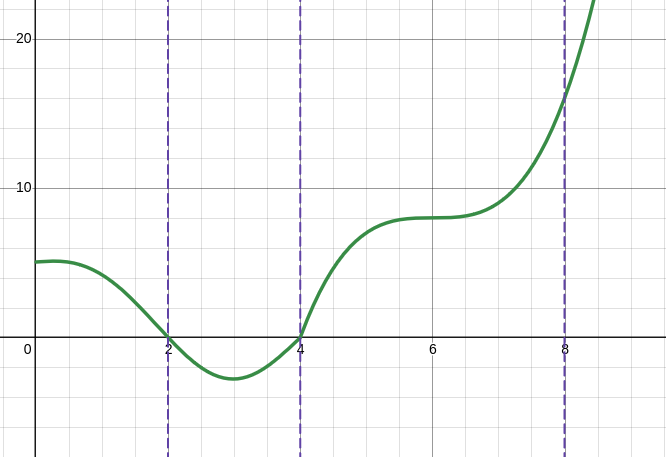
\includegraphics[width=3in]{numeric-integral.png}

	The graph above is of the function $f$. Marked on the graph are the intervals
	$A=[0,2]$, $B=[2,4]$, and $C=[4,8]$. We are interested in the quantity $\displaystyle I=\int_0^8 f(x)\,\mathrm d x$.
	\begin{parts}
		\item On each interval, identify whether left/right/midpoint/trapezoid approximations will produce an
		\begin{enumerate}
			\item Underestimate 
			\item Overestimate 
			\item Cannot be determined
		\end{enumerate}

		\item Is there any interval where you're confident that Simpson's rule would produce 
		an over/under estimate?

		\item Come up with a strategy (i.e., a choice of integration method for each interval)
		that gives the best possible upper and lower bounds for $I$.

	\end{parts}
\end{slide}

\begin{slide}
	\question
	Given an interval $[a,b]$ the midpoint-rule (with one interval) says to use $(b-a)f(0.5a+0.5b)$ as an estimate
	for $I=\displaystyle \int_a^b f(x)\,\mathrm d x$.

	A \emph{biased} midpoint rule with bias $\alpha\in[0,1]$ uses $(b-a)f(\alpha a+(1-\alpha)b)$
	as an estimate for $I$.

	\begin{parts}
		\item Is there a bias $\alpha$ so that with a single partition, $\displaystyle\int_0^1 x^2\,\mathrm d x$ is \emph{perfectly} approximated? If so, what is the bias?

		\item Is there a bias $\alpha$ so that with \emph{two} partitions, $\displaystyle \int_0^1 x^2\,\mathrm d x$ is \emph{perfectly} approximated? If so, what is the bias?

		\item How do your biases compare with the standard midpoint rule?
	\end{parts}
\end{slide}

\begin{slide}
	\question

	\begin{parts}
		\item Explain to your table: What is the difference between a sequence and a series?
		\item How can you produce a sequence from a series?
		\item How can you produce a series from a sequence?
		\item Give an example of a bounded sequence that when summed produces an unbounded series.
	\end{parts}
\end{slide}

\begin{slide}
	\question
	Define the sequence $a_n$ by $
		a_n = \sin(\pi n)$
	and the function $f$ by $f(x) = \sin(\pi x)$.

	\begin{parts}
		\item Find $\displaystyle \lim_{n\to\infty} a_n$, if it exists.
		\item Find $\displaystyle \lim_{x\to\infty} f(x)$, if it exists.

		\item What is the difference between a sequence and a function.
	\end{parts}
\end{slide}

\begin{slide}
	\question
	Define \[
		a_n = \frac{4+n}{2+n} \qquad b_n = \frac{(-1)^n}{n^2}
	\]
	for $n\geq 1$.

	\begin{parts}
		\item If $a_n$ and $b_n$ define sequences, what values can $n$ take on? (E.g., any number in $\R$, any number in $\Z$, etc.)
		\item Make a plot of $a_n$ vs. $n$ and $b_n$ vs. $n$.
		\item Which sequences (out of $a_n$ and $b_n$) are (i) bounded above, (ii) bounded below,
		(iii) strictly increasing, (iv) strictly decreasing, (v) alternating.

		\item Define $c_n=a_{n-1} + b_{2n}$ for $n\geq 2$. Find a formula for $c_n$.

		\item Based on your answer to Part 3, will $c_n$ be bounded above or below?	Neither?

		\item Find $\displaystyle \lim_{n\to\infty} c_n$.
	\end{parts}
\end{slide}

\begin{slide}
	\question
	Let $a_n$ (for $n\geq 1$) be a sequence and define 
	\[
	S_n = \sum_{i=1}^n a_n.
	\]
	Let $S_\infty = \lim_{n\to\infty } S_n$.

	\begin{parts}
		\parbox{\textwidth}{
		\item Which of the following statements must be true?

		\begin{enumerate}
			\item If $|a_n| \geq 1$ for all $n$, then $S_n$ converges.
			\item If $|a_n| \leq 1$ for all $n$, then $S_n$ converges.
			\item If $|S_n| \geq 1$ for all $n$, then $a_n$ diverges.
			\item If $|S_n| \leq 1$ for all $n$, then $a_n$ diverges.
			\item If $a_n\to 0$ then $S_n$ converges.

		\end{enumerate}
		}

		\bigskip
		\bigskip
		\item If you switch \emph{converges} $\leftrightarrow$ \emph{diverges},
		which statements change their truth value? (I.e., switch from being true to false or
		false to true.)
	\end{parts}
\end{slide}

\begin{slide}
	\question
	Consider the function $f(x)=1/x$, the sequence $a_n=1/n$ and 
	the sequence of partial sums $\displaystyle S_n = \sum_{i=1}^n a_i$.

	In this question we want to get bounds on the \emph{series}
	\[
		\sum_{i=1}^\infty a_i
	\]
	\begin{parts}
		\item Use $\Sigma$-notation to write down a formula for the left-endpoint approximation of
		$\displaystyle \int_1^n \frac{1}{x}\,\mathrm d x$ using a partition
		whose intervals are width $1$.

		\bigskip
		\bigskip
		\bigskip
		\item Use $\Sigma$-notation to write down a formula for the right-endpoint approximation of
		$\displaystyle \int_1^n \frac{1}{x}\,\mathrm d x$ using a partition
		whose intervals are width $1$.
		\item Use the actual value of $\displaystyle \int_1^n \frac{1}{x}\,\mathrm d x$ to give upper and lower bounds for $S_n$.
		\item Does $S_n$ converge or diverge? Explain.
	\end{parts}
\end{slide}

\begin{slide}
	\question
	Consider the function $f(x)=1/x^2$, the sequence $a_n=1/n^2$ and 
	the sequence of partial sums $\displaystyle S_n = \sum_{i=1}^n a_i$.

	In this question we want to get bounds on the \emph{series}
	\[
		\sum_{i=1}^\infty a_i
	\]
	\begin{parts}
		\item Use $\Sigma$-notation to write down a formula for the left-endpoint approximation of
		$\displaystyle \int_1^n \frac{1}{x^2}\,\mathrm d x$ using a partition
		whose intervals are width $1$.
		
		\bigskip
		\bigskip
		\bigskip
		\item Use $\Sigma$-notation to write down a formula for the right-endpoint approximation of
		$\displaystyle \int_1^n \frac{1}{x^2}\,\mathrm d x$ using a partition
		whose intervals are width $1$.
		\item Use the actual value of $\displaystyle \int_1^n \frac{1}{x^2}\,\mathrm d x$ to give upper and lower bounds for $S_n$.
		\item Does $S_n$ converge or diverge? Explain.
		\item Conjecture about the convergence of $\displaystyle \sum_{i=1}^\infty i^{\alpha}$ for $\alpha> 0$. Can you justify your answer by comparing with known integrals?
	\end{parts}
\end{slide}

\begin{slide}
	\question
	Let
	\[
		a_n =\frac{1}{\sqrt{n}}\qquad b_n=\frac{1}{n^3}\qquad c_n=e^{-n}
		\qquad d_n=e^{-n^2}
	\]
	and consider the corresponding sequences of partial sums $A_n$, $B_n$,
	$C_n$, and $D_n$. (I.e., $\displaystyle A_n=\sum_{i=1}^n a_n$, etc.)

	\begin{parts}
		\item Use a comparison with known integrals to decide 
		the convergence of $A_n$, $B_n$, $C_n$.
		\item Can you decide the convergence of $D_n$ using a comparison to
		a known integral? Explain.
	\end{parts}
\end{slide}

\begin{slide}
	\question
	Consider the function $f(x)=\sin(x)$.

	\begin{parts}
		\item Write down $T_k(x)$, the $k$th Taylor approximation to 
		$f$ centered at $0$. You may use ``$\cdots$'' notation or $\Sigma$-notation. 

		\item Write down, using $\Sigma$-notation, $T(x)$, the Taylor series
		for $f$ centered at $0$.

		\item In general a Taylor series may be written as $\displaystyle 
		\sum_{n=0}^\infty a_n \frac{x^{n}}{n!}$, where $a_n$ is a sequence.
		Find $a_n$ in this case.

		\item Let $R_k(x)=f(x)-T_k(x)$. Find an expression for $R_k(x)$
		using Taylor's Remainder Theorem. Use your expression to find an upper bound for $|R_k(x)|$ (Hint: your bound may depend on $x$).
	
		\item Using the fact that for any $\alpha\in \R$, 
		$\displaystyle \lim_{n\to\infty} \frac{\alpha^n}{n!}=0$, 
		find $\displaystyle \lim_{k\to\infty} R_k(x)$.

		\item For which $x$ is $f(x)=T(x)$? Justify your answer.
	\end{parts}
\end{slide}

\begin{slide}
	\question
	Consider the function $g(x)=\frac{1}{1-x}$. The $k$th Taylor approximation
	of $g$ centered at $0$ is 
	\[
	T_k(x)=\sum_{i=0}^k x^k
	\]
	and the remainder $R_k(x)=g(x)-T_k(x)$ satisfies 
	\[
		|R_k(x)| \leq \frac{1}{1-x}\left(\frac{x}{1-x}\right)^{k+1}
	\]
	when $x\geq 0$ and
	\[
		|R_k(x)| \leq x^{k+1}
	\]
	when $x< 0$.

	\bigskip
	\bigskip
	\bigskip
	\begin{parts}
		\item For which $x$ is $\lim_{k\to\infty}R_k(x)=0$?

		\item Let $T(x)$ be the Taylor series for $g$ centered at $0$.
		For which $x$ can you guarantee that $g(x)=T(x)$?

		\item Use the following Desmos link to numerically answer the question: for which $x$ does $g(x)=T(x)$?

		{\small\url{https://www.desmos.com/calculator/yi4qczkxqn}}

		\item Does your answer to the previous part contradict Taylor's remainder theorem?

	\end{parts}
\end{slide}

\begin{slide}
	\question
	Let $f(x)=\sin(x)$ and let 
	\[
		T(x)=\sum_{n=0}^\infty (-1)^{n}\frac{x^{2n+1}}{(2n+1)!}
	\]
	be the Taylor series for $f$ centered at $0$. We know that
	$f(x)=T(x)$ for all $x\in \R$.

	\begin{parts}
		\item Find a series representation for $g_1(x)=f(2x)$ (without 
		computing any derivatives).
		\item Find a series representation for $g_2(x)=f(x^2)$.
		\item Use WolframAlpha to integrate $g_2$. Does WolframAlpha's solution make sense?
		\item Compute $g_3(x)=\displaystyle \int g_2(x)\,\mathrm d x$ by integrating your series for $g_2(x)$ term by term. What should you do with the constants of integration?
		\item For which $x$ do you expect $g_3(x)$ to be valid? Explain.
		\item When would it be advantageous to integrate a Taylor series term by term instead of integrating the original function? Explain.
	\end{parts}
\end{slide}

\begin{slide}
	\question
	Let $f(x)=\frac{1}{1-x}$ and let 
	\[
		T(x)=\sum_{n=0}^\infty x^n
	\]
	be the Taylor series for $f$ centered at $0$. We know that
	$f(x)=T(x)$ for all $x\in (-1,1)$.

	\begin{parts}
		\item Find a series representation for $g_1(x)=f(2x)$ (without 
		computing any derivatives).
		\item For which $x$ do you expect your series for $g_1(x)$ to be valid (i.e. to equal
		$f(2x)$? Explain.
		\item Find a series representation for $g_2(x)=f(x^2)$.
		\item Compute $g_3(x)=\displaystyle \int g_2(x)\,\mathrm d x$ by integrating your series for $g_2(x)$ term by term. 
		\item For which $x$ do you expect $g_3(x)$ to be valid? Explain.
	\end{parts}
\end{slide}

\begin{slide}
	\question
	The function $f$ has a Taylor series centered at $0$ of the form
	\[
		T(x)=\frac{1}{2}+\frac{x}{3}-\frac{x^2}{4}+\frac{x^3}{5}-\frac{x^4}{6}+\cdots.
	\]

	\begin{parts}
		\item Express $T$ using $\Sigma$-notation.
		\item Find a series representation for $f'(x)$ and $\int f(x)\,\mathrm d x$.
		\item Modify the following Desmos link and make a conjecture as to which range 
		of $x$ values is $f(x)=T(x)$.

		\url{https://www.desmos.com/calculator/try63qzvo5}
	\end{parts}
\end{slide}

\begin{slide}
	\question
	Recall 
	\[
		\sin x = \sum_{n=0}^\infty (-1)^n\frac{x^{2n+1}}{(2n+1)!}
		\qquad
		\cos x = \sum_{n=0}^\infty (-1)^n\frac{x^{2n}}{(2n)!}
	\]

	Let $f(x)=\cos(\sqrt{x})$.

	\begin{parts}
		\item Write down a Taylor series for $f$.

		\emph{Hint: if your derivatives get too messy, try a different strategy.}

		\item Find $f^{(10)}(0)$.
		
		\item For what $x$ is your series valid? Explain.s

		\item Using Desmos, make a conjecture as to which range of $x$ your series converges.

		\url{https://www.desmos.com/calculator/try63qzvo5}

		\item Let $T$ be a Taylor series for an unknown function $f$.
		If a Taylor series $T$ converges at a value $x_0$, must it be true that $T(x_0)=f(x_0)$?
		Explain. 

	\end{parts}
\end{slide}

%\begin{slide}
%	\question
%	In the model \textbf{M$_1$}, we assumed the starfish had $K$ children at one point during the year.
%
%	\begin{parts}
%		\item Create a model \textbf{M$_n$} where the starfish are assumed to have $K/n$ children $n$ times per year (at regular intervals).
%		\item Simulate the models \textbf{M$_1$}, \textbf{M$_2$}, \textbf{M$_3$} in Excel. Which grows fastest?
%		\item What happens to \textbf{M$_n$} as $n\to\infty$?
%	\end{parts}
%
%\end{slide}
%
%\begin{slide}
%	\question
%	Exploring \textbf{M$_n$}
%
%	We can rewrite the assumptions of \textbf{M$_n$} as follows:
%	\begin{itemize}
%		\item At time $t$ there are $P_n(t)$ starfish.
%		\item $P_n(0)=10$
%		\item During the time interval $(t, t+1/n)$ there will be (on average) $K/n$ new children per starfish.
%	\end{itemize}
%
%	\begin{parts}
%		\item Write an expression for $P_n(t+1/n)$ in terms of $P_n(t)$.
%		\item Write an expression for $\Delta P_n$, the change in population from time $t$ to $t+\Delta t$.
%		\item Write an expression for $\frac{\Delta P_n}{\Delta t}$.
%		\item Write down a \emph{differential equation} relating $P'(t)$ to $P(t)$ where $\displaystyle P(t)=\lim_{n\to\infty} P_n(t)$.
%	\end{parts}
%\end{slide}
%
%\begin{slide}
%	\question
%	Recall the model \textbf{M$_1$} defined by
%	\begin{itemize}
%		\item $P_1(0)=10$
%		\item $P_1(t+1) = KP(t)$ for $t\geq 0$ years and $K=1.1$.
%	\end{itemize}
%	Define the model \textbf{M$_\infty$} by
%	\begin{itemize}
%		\item $P(0)=10$
%		\item $P'(t) = kP(t)$.
%	\end{itemize}
%
%
%	\begin{parts}
%		\item If $k=K=1.1$, does the model \textbf{M$_\infty$} produce the same population estimates as \textbf{M$_1$}?
%	\end{parts}
%
%	\vspace*{1in}
%\end{slide}
%
%\begin{slide}
%	\question
%	Suppose that the estimates produced by \textbf{M$_1$} agree with the actual (measured) population of starfish.
%
%	Fill out the table indicating which models have which
%	properties.
%
%	\begin{center}
%	\begin{tabular}{|c|c|c|c|}
%		\hline
%		Model & Accuracy & Explanatory & (your favourite property)\\
%		\hline
%		\textbf{M$_1$} & \phantom{$\displaystyle\int$} & & \\
%		\hline
%		\textbf{M$_1^*$} &\phantom{$\displaystyle\int$} & & \\
%		\hline
%		\textbf{M$_\infty$} &\phantom{$\displaystyle\int$} & & \\
%		\hline
%	\end{tabular}
%	\end{center}
%\end{slide}
%
%\begin{slide}
%	\question
%	Recall the model \textbf{M$_1$} defined by
%	\begin{itemize}
%		\item $P_1(0)=10$
%		\item $P_1(t+1) = KP(t)$ for $t\geq 0$ years and $K=1.1$.
%	\end{itemize}
%	Define the model \textbf{M$_\infty$} by
%	\begin{itemize}
%		\item $P(0)=10$
%		\item $P'(t) = kP(t)$.
%	\end{itemize}
%
%	\begin{parts}
%		\item Suppose that \textbf{M$_1$} accurately predicts the population. Can you find a value of $k$ so that \textbf{M$_\infty$}
%		accurately predicts the population?
%		%\item What are some advantages and disadvantages of the models \textbf{M$_1$} and \textbf{M$_\infty$}?
%	\end{parts}
%
%	\vspace*{1in}
%\end{slide}
%
%\begin{slide}
%	\question
%	After more observations, scientists notice a seasonal effect on starfish. They propose a new model called \textbf{S}:
%	\begin{itemize}
%		\item $P(0)=10$
%		\item $P'(t) = k\cdot P(t)\cdot |\sin(2\pi t)|$
%	\end{itemize}
%	
%	\begin{parts}
%		\item What can you tell about the population (without trying to compute it)?
%		\item Assuming $k=1.1$, estimate the population after 10 years.
%		\item Assuming $k=1.1$, estimate the population after 10.3 years.
%	\end{parts}
%\end{slide}
%
%\begin{slide}
%	\question
%	Consider the following argument for the population model \textbf{S} where
%	$P'(t)=P(t)\cdot\abs{\sin(2\pi t)}$ with $P(0)=10$:
%	\begin{quote}
%		\color{blue}
%		At $t=0$, the change in population $\approx P'(0)=0$, so
%		\[
%			P(1) \approx P(0)+P'(0)\cdot 1 = P(0)=10.
%		\]
%		At $t=1$, the change in population $\approx P'(1)=0$, so
%		\[
%			P(2) \approx P(1)+P'(1)\cdot 1 = P(0)=10.
%		\]
%		And so on.
%
%		So, the population of starfish remains constant.
%	\end{quote}
%	
%	%\vspace*{.1in}
%	\begin{parts}
%		\item Do you believe this argument? Can it be improved?
%		\item Simulate an improved version using a spreadsheet.
%	\end{parts}
%	\vspace*{1.5in}
%\end{slide}
%
%\begin{slide}
%	\question
%	(Simulating \textbf{M$_\infty$} with different $\Delta$s)
%	
%	\begin{center}
%	\begin{tabular}{l|l|l|l}
%		Time & Pop. ($\Delta=0.1$) & Time & Pop. ($\Delta=0.2$)\\
%		\hline
%		0.0&	10&		0.0&	10\\
%		0.1&	11.1&		0.2&	12.2\\
%		0.2&	12.321&		0.4&	14.884\\
%		0.3&	13.67631&	0.6&	18.15848\\
%		0.4&	15.1807041&	0.8&	22.1533456
%	\end{tabular}
%	\end{center}
%
%	\begin{parts}
%		\item Compare $\Delta=0.1$ and $\Delta=0.2$. Which approximation grows faster?
%		\item Graph the population estimates for $\Delta=0.1$ and $\Delta=0.2$ on the same plot. What does the graph show?
%
%		\vspace{1cm}
%		\item What $\Delta$s give the largest estimate for the population at time $t$?
%		\item Is there a limit as $\Delta\to 0$?
%	\end{parts}
%\end{slide}
%
%\begin{slide}
%	(Simulating \textbf{M$_\infty$} with different $\Delta$s)
%	
%	% https://www.desmos.com/calculator/x7qbgv6mkc
%	\includegraphics[width=2.5in]{compare-deltas.png}
%
%	\begin{parts}
%		\item Compare $\Delta=0.1$ and $\Delta=0.2$. Which approximation grows faster?
%		\item Graph the population estimates for $\Delta=0.1$ and $\Delta=0.2$ on the same plot. What does the graph show?
%
%		\vspace{1cm}
%		\item What $\Delta$s give the largest estimate for the population at time $t$?
%		\item Is there a limit as $\Delta\to 0$?
%	\end{parts}
%\end{slide}
%
%\begin{slide}
%	\question
%	\label{many-models}
%	Consider the following models for starfish growth
%	\begin{itemize}
%		\item[\textbf{M}] \# new children per year $\sim$ current population
%		\item[\textbf{N}] \# new children per year $\sim$ current population times resources available per individual
%		\item[\textbf{O}] \# new children per year $\sim$ current population times the fraction of total resources remaining
%	\end{itemize}
%
%	\begin{parts}
%		\item Guess what the population vs. time curves look like for each model. \label{model-guess-part}
%		\item Create a differential equation for each model.
%		\item Simulate population vs. time curves for each model (but pick a common initial population).
%	\end{parts}
%\end{slide}
%
%\begin{slide}
%	\question
%	Recall the models
%	\begin{itemize}
%		\item[\textbf{M}] \# new children per year $\sim$ current population
%		\item[\textbf{N}] \# new children per year $\sim$ current population times resources available per individual
%		\item[\textbf{O}] \# new children per year $\sim$ current population times the fraction of total resources remaining
%	\end{itemize}
%
%	\begin{parts}
%		\item Determine which population grows fastest in the short term and which grows fastest in the long term.
%		\item Are some models more sensitive to your choice of $\Delta$ when simulating?
%		\item Are your simulations for each model consistently underestimates? Overestimates?
%		\item Compare your simulated results with your guesses from question \ref{many-models}.\ref{model-guess-part}.
%		What did you guess correctly? Where were you off the mark?
%	\end{parts}
%\end{slide}
%
%%
%% Hours 7-9
%%
%
%
%\begin{slide}
%	\question
%	A simple model for population growth has the form
%	\[
%		P'(t) = bP(t)
%	\]
%	where $b$ is the \emph{birth rate}.
%
%	\begin{parts}
%		\item Create a better model for population that includes both births and deaths.
%	\end{parts}
%\end{slide}
%
%\begin{slide}
%	\question
%	\emph{Lotka-Volterra Predator-Prey} models predict two populations, $F$ (foxes) and $R$ (rabbits), simultaneously. They take the form
%	\begin{align*}
%		F'(t) &= (B_F - D_F)\cdot F(t)\\
%		R'(t) &= (B_R - D_R)\cdot R(t)
%	\end{align*}
%	where $B_{?}$ stands for births and $D_{?}$ stands for deaths.
%
%	We will assume:
%	\vspace{-.3cm}
%	\begin{itemize}
%		\item Foxes die at a constant rate.
%		\vspace{-.1cm}
%		\item Foxes mate when food is plentiful.
%		\vspace{-.1cm}
%		\item Rabbits mate at a constant rate.
%		\vspace{-.1cm}
%		\item Foxes eat rabbits.
%	\end{itemize}
%
%	\bigskip
%	\begin{parts}
%		\item Speculate on when $B_F$, $D_F$, $B_R$, and $D_R$ would be at their maximum(s)/minimum(s), given our assumptions.
%		\item Come up with appropriate formulas for $B_F$, $B_R$, $D_F$, and $D_R$.
%	\end{parts}
%	\bigskip
%	\bigskip
%	\bigskip
%	\bigskip
%	\bigskip
%	\bigskip
%	\phantom{x}
%\end{slide}
%
%\begin{slide}
%	\question
%	Suppose the population of $F$ (foxes) and $R$ (rabbits) evolves over time following the rule
%	\begin{align*}
%		F'(t) &= (0.01\cdot R(t) - 1.1)\cdot F(t)\\
%		R'(t) &= (1.1 - 0.1\cdot F(t))\cdot R(t)
%	\end{align*}
%
%	\begin{parts}
%		\item Simulate the population of foxes and rabbits with a spreadsheet.
%		\item Do the populations continue to grow/shrink forever? Are they cyclic?
%		\item Should the humps/valleys in the rabbit and fox populations be in phase? Out of phase?
%	\end{parts}
%\end{slide}
%
%\begin{slide}
%	\question
%	% https://utoronto-my.sharepoint.com/:x:/g/personal/jason_siefken_utoronto_ca/Eay4QOMvy7lNr5pOKRv22NgBLGUw7qMpSCShUjeAdrhsHQ?e=bpg4CP
%	Open the spreadsheet
%
%	\url{https://uoft.me/foxes-and-rabbits}
%
%	which contains an Euler approximation for the Foxes and Rabbits population.
%	\begin{align*}
%		F'(t) &= (0.01\cdot R(t) - 1.1)\cdot F(t)\\
%		R'(t) &= (1.1 - 0.1\cdot F(t))\cdot R(t)
%	\end{align*}
%
%	\begin{parts}
%		\item Is the max population of the rabbits over/under estimated? Sometimes over, sometimes under?
%		\item What about the foxes?
%		\item What about the min populations?
%	\end{parts}
%\end{slide}
%
%\begin{slide}
%	\question
%	% https://utoronto-my.sharepoint.com/:x:/g/personal/jason_siefken_utoronto_ca/Eay4QOMvy7lNr5pOKRv22NgBLGUw7qMpSCShUjeAdrhsHQ?e=bpg4CP
%	Open the spreadsheet
%
%	\url{https://uoft.me/foxes-and-rabbits}
%
%	which contains an Euler approximation for the Foxes and Rabbits population.
%	\begin{align*}
%		F'(t) &= (0.01\cdot R(t) - 1.1)\cdot F(t)\\
%		R'(t) &= (1.1 - 0.1\cdot F(t))\cdot R(t)
%	\end{align*}
%
%	\SavedDefinitionRender{ComponentGraphAndPhasePlane}
%
%	\begin{parts}
%		\item Plot the Fox vs.~Rabbit population in the \emph{phase plane}. 
%		\item Should your plot show a closed curve or a spiral?
%		\item What ``direction'' do points move along the curve as time increases? Justify by referring to the model.
%		\item What is easier to see from plots in the phase plane than from component graphs (the graphs of
%		fox and rabbit population vs. time)?
%	\end{parts}
%\end{slide}
%
%\begin{slide}
%	\question
%	% https://utoronto-my.sharepoint.com/:x:/g/personal/jason_siefken_utoronto_ca/Eay4QOMvy7lNr5pOKRv22NgBLGUw7qMpSCShUjeAdrhsHQ?e=bpg4CP
%	Open the spreadsheet
%
%	\url{https://uoft.me/foxes-and-rabbits}
%
%	which contains an Euler approximation for the Foxes and Rabbits population.
%	\begin{align*}
%		F'(t) &= (0.01\cdot R(t) - 1.1)\cdot F(t)\\
%		R'(t) &= (1.1 - 0.1\cdot F(t))\cdot R(t)
%	\end{align*}
%
%	\SavedDefinitionRender{EquilibriumSolution}
%
%	\begin{parts}
%		\item By changing initial conditions, what is the ``smallest'' curve you can get in the phase plane? What happens at
%		those initial conditions?
%		\item What should $F'$ and $R'$ be if $F$ and $R$ are \emph{equilibrium solutions}?
%		\item How many equilibrium solutions are there for the fox-and-rabbit system? Justify your answer.
%		\item What do the equilibrium solutions look like in the phase plane? What about their component graphs?
%	\end{parts}
%\end{slide}
%
%\begin{slide}
%	\question
%	Recall the logistic model for starfish growth:
%	\begin{itemize}
%		\item[\textbf{O}] \# new children per year $\sim$ current population times the fraction of total resources remaining
%	\end{itemize}
%	which can be modeled with the equation
%	\[
%		P'(t) = k\cdot P(t)\cdot \left(1-\tfrac{R_i}{R}\cdot P(t)\right)
%	\]
%	where 
%	\begin{itemize}
%		\item $P(t)$ is the population at time $t$
%		\item $k$ is a constant of proportionality 
%		\item $R$ is the total number of resources
%		\item $R_i$ is the resources that one starfish wants to consume
%	\end{itemize}
%
%	Use $k=1.1$, $R=1$, and $R_i=0.1$ unless instructed otherwise.
%
%	\begin{parts}
%		\item What are the equilibrium solutions for model \textbf{O}?
%		\item What does a ``phase plane'' for model \textbf{O} look like? What do graphs of equilibrium solutions look like?
%		\item Classify the behaviour of solutions that lie \emph{between} the equilibrium solutions. E.g., are they increasing, decreasing, oscillating?
%	\end{parts}
%\end{slide}
%
%\begin{slide}
%	\question
%
%	\SavedDefinitionRender{ClassificationOfEquilibria}
%
%	\SavedDefinitionRender{ClassificationOfEquilibriaFormal}
%\end{slide}
%
%\begin{slide}
%	\SavedDefinitionRender{ClassificationOfEquilibria}
%
%	Let
%	\[
%		F'(t) =\ ?
%	\]
%	be an unknown differential equation with equilibrium solution $f(t)=1$.
%
%	\begin{parts}
%		\item Draw an example of what solutions might look like if $f$ is \emph{attracting}.
%		\item Draw an example of what solutions might look like if $f$ is \emph{repelling}.
%		\item Draw an example of what solutions might look like if $f$ is \emph{stable}.
%		\item Could $f$ be stable but \emph{not} attracting?
%	\end{parts}
%\end{slide}
%
%\begin{slide}
%	\question
%	
%	\SavedDefinitionRender{ClassificationOfEquilibria}
%	
%	Recall the starfish population model \textbf{O} given by
%	\[
%		P'(t) = k\cdot P(t)\cdot \left(1-\tfrac{R_i}{R}\cdot P(t)\right)
%	\]
%	Use $k=1.1$, $R=1$, and $R_i=0.1$ unless instructed otherwise.
%
%
%	\begin{parts}
%		\item Classify the equilibrium solutions for model \textbf{O} as attracting/repelling/stable/unstable/semi-stable.
%		\item Does changing $k$ change the nature of the equilibrium solutions? How can you tell?
%	\end{parts}
%\end{slide}
%
%%
%% Hours 10-12
%%
%
%\begin{slide}
%	% https://www.desmos.com/calculator/ghavqzqqjn
%
%	\question
%	
%	\begin{center}
%	\includegraphics[width=2.5in]{slope-field-for-O.png}
%	\end{center}
%
%	A \emph{slope field} is a plot of small segments of tangent lines
%	to solutions of a differential equation at different initial conditions.
%	
%	On the left is a slope field for model \textbf{O}, available at
%
%	\url{https://www.desmos.com/calculator/ghavqzqqjn}
%
%	\begin{parts}
%		\item If you were sketching the slope field for model \textbf{O} by hand, what line would you sketch
%		(a segment of) at $(5,3)$? Write an equation for that line.
%		\item How can you recognize equilibrium solutions in a slope field?
%		\item Give qualitative descriptions of different solutions to the \emph{differential equation} used in model \textbf{O} (i.e., use words to describe them). Do all
%		of those solutions make sense in terms of \emph{model \textbf{O}}?
%	\end{parts}
%\end{slide}
%
%\begin{slide}
%	% https://www.desmos.com/3d/kvyztvmp0g
%
%	\question
%	
%	\begin{center}
%		\includegraphics[width=2in]{slope-field-3d.png}
%	\end{center}
%
%	3d slope fields are possible, but hard to interpret.
%
%	On the left is a slope field for the Foxes--Rabbits model.
%
%	\url{https://www.desmos.com/3d/kvyztvmp0g}
%
%	\begin{parts}
%		\item What are the three dimensions in the plot?
%		\item What should the graph of an equilibrium solution look like?
%		\item What should the graph of a typical solution look like?
%		\item What are ways to simplify the picture so we can more easily analyze solutions?
%	\end{parts}
%\end{slide}
%
%
%\begin{slide}
%	% https://www.desmos.com/calculator/wdgtznxndp
%	%
%	% Without Euler's built in:
%	% https://www.desmos.com/calculator/vrk0q4espx
%
%	\question
%	
%	\begin{center}
%		\includegraphics[width=2.5in]{phase-portrait-foxes-wolves.png}
%	\end{center}
%
%
%	\SavedDefinitionRender{PhasePortrait}
%
%	On the left is a phase portrait for the Foxes--Rabbits model.
%
%	\url{https://www.desmos.com/calculator/vrk0q4espx}
%
%	\begin{parts}
%		\item What do the $x$ and $y$ axes correspond to?
%		\item Identify the equilibria in the phase portrait. What are the lengths of the vectors at those points?
%		\item Classify each equilibrium as stable/unstable.
%		\item Copy and paste data from your simulation spreadsheet into the Desmos plot. Does the resulting
%		curve fit with the picture?
%		%\item Why is the vector at $(5,100)$ longer than the vector at $(10,100)$? Justify numerically.
%	\end{parts}
%\end{slide}
%
%\begin{slide}
%	% https://www.desmos.com/calculator/wdgtznxndp
%	%
%	% Without Euler's built in:
%	% https://www.desmos.com/calculator/vrk0q4espx
%
%	\question
%	Sketch your own vector field where the corresponding system of differential equations:
%
%	\begin{parts}
%		\item Has an attracting equilibrium solution.
%		\item Has a repelling equilibrium solution.
%		\item Has no equilibrium solutions.
%	\end{parts}
%\end{slide}
%
%\begin{slide}
%	% https://www.desmos.com/calculator/ghavqzqqjn
%
%	\question
%	
%	\begin{center}
%	\includegraphics[width=2.5in]{slope-field-for-O.png}
%	\end{center}
%
%	Recall the slope field for model \textbf{O}.
%
%	\begin{parts}
%		\item What would a phase portrait for model \textbf{O} look like? Draw it.
%		\item Where are the arrows the longest? Shortest?
%		\item How could you tell from a 1d phase portrait whether an equilibrium solution is
%		attracting/repelling/etc.?
%	\end{parts}
%\end{slide}
%
%\begin{slide}
%	%
%	% Completed phase portrait in desmos:
%	% https://www.desmos.com/calculator/tvjag852ja
%	\question
%	\label{q-phase}
%	The following differential equation models the life cycle of a tree.
%	In the model
%	\begin{itemize}
%		\item $H(t)\ =$ height (in meters) of tree trunk at time $t$
%		\item $A(t)\ =$ surface area (in square meters) of all leaves at time $t$
%	\end{itemize}
%	\begin{align*}
%		H'(t) &= 0.3\cdot A(t)-b\cdot H(t)\\
%		A'(t) &= -0.3\cdot (H(t))^2 + A(t)
%	\end{align*}
%	and $0 \leq b \leq 2$
%
%	\bigskip
%	\phantom{x}
%	\begin{parts}
%		\item 
%		\label{part-phase}
%		Modify 
%
%		{\small
%		\url{https://www.desmos.com/calculator/vrk0q4espx}
%		}
%
%		to make a phase portrait for the tree model.
%		\item What do equilibrium solutions mean in terms of tree growth?
%		\item For $b=1$ what are the equilibrium solution(s)?
%	\end{parts}
%	\bigskip
%	\phantom{x}
%\end{slide}
%
%\begin{slide}
%	%
%	% Completed phase portrait in desmos:
%	% https://www.desmos.com/calculator/tvjag852ja
%	\question
%	The following differential equation models the life cycle of a tree.
%	In the model
%	\begin{itemize}
%		\item $H(t)\ =$ height (in meters) of tree trunk at time $t$
%		\item $A(t)\ =$ surface area (in square meters) of all leaves at time $t$
%	\end{itemize}
%	\begin{align*}
%		H'(t) &= 0.3\cdot A(t)-b\cdot H(t)\\
%		A'(t) &= -0.3\cdot (H(t))^2 + A(t)
%	\end{align*}
%	and $0 \leq b \leq 2$
%
%	\bigskip
%	\phantom{x}
%	\begin{parts}
%		\item Fix a value of $b$ and use a spreadsheet to simulate some solutions with different initial conditions.
%		Plot the results on your phase portrait from \ref{q-phase}.\ref{part-phase}.
%		\item What will happen to a tree with $(H(0), A(0))=(20,10)$? Does this depend on $b$?
%		\item What will happen to a tree with $(H(0), A(0))=(10,10)$? Does this depend on $b$?
%	\end{parts}
%	\bigskip
%	\phantom{x}
%\end{slide}
%
%\begin{slide}
%	\question
%	The tree model
%	\begin{align*}
%		H'(t) &= 0.3\cdot A(t)-b\cdot H(t)\\
%		A'(t) &= -0.3\cdot (H(t))^2 + A(t)
%	\end{align*}
%	was based on the premises
%	\begin{itemize}[leftmargin=3em]
%		\item[ $P_{\text{height 1}}$] CO$_2$ is absorbed by the leaves and turned directly into trunk height.
%		\item[ $P_{\text{height 2}}$] The tree is in a swamp and constantly sinks at a speed proportional to its height.
%		\item[ $P_{\text{leaves 1}}$] Leaves grow proportionality to the energy available.
%		\item[ $P_{\text{energy 1}}$] The tree gains energy from the sun proportionally to the leaf area.
%		\item[ $P_{\text{energy 2}}$] The tree loses energy proportionally to the square of its height.
%		%\item[ $P_{\text{energy 1}}$] The tree absorbs energy from the sun proportionality to the leaf area.
%		%\item[ $P_{\text{energy 2}}$] It costs energy proportional to the square of the height for the tree to maintain its current size.
%	\end{itemize}
%
%	\begin{parts}
%		\item How are the premises expressed in the differential equations?
%		\item What does the parameter $b$ represent (in the real world)?
%		\item Applying Euler's method to this system shows solutions that pass from the 1st to 4th quadrants of the phase plane.
%			Is this realistic? Describe the life cycle of such a tree?
%	\end{parts}
%\end{slide}
%
%\begin{slide}
%	\question
%	Recall the tree model
%	\begin{align*}
%		H'(t) &= 0.3\cdot A(t)-b\cdot H(t)\\
%		A'(t) &= -0.3\cdot (H(t))^2 + A(t)
%	\end{align*}
%
%	\begin{parts}
%		\item Find all equilibrium solutions for $0\leq b\leq 2$.
%		\item For which $b$ does a tree have the possibility of living forever? If the wind occasionally blew off a few random leaves,
%		would that change your answer?
%		\item
%		Find a value $b_5$ of $b$ so that there is an equilibrium with $H=5$.
%
%		Find a value $b_{12}$ of $b$ so that there is an equilibrium with $H=12$.
%		
%		\item
%		Predict what happens to a tree near equilibrium in condition $b_5$ and a tree near equilibrium in condition $b_{12}$.
%
%	\end{parts}
%\end{slide}
%
%%
%% Hours 13-14
%%
%
%\begin{slide}
%	\question
%	Consider the system of differential equations
%	\begin{align*}
%		x'(t) &= x(t)\\
%		y'(t) &= 2y(t)
%	\end{align*}
%
%	\begin{parts}
%		\item Make a phase portrait for the system.
%
%		{\small \url{https://www.desmos.com/calculator/h3wtwjghv0}}
%		\item What are the equilibrium solution(s) of the system?
%		\item 
%		Find a formula for $x(t)$ and $y(t)$ that satisfy the initial conditions $(x(0), y(0))=(x_0, y_0)$.
%		\item Let $\vec r(t)=(x(t),y(t))$. Find a matrix $A$ so that the differential equation can be equivalently expressed
%		as
%		\[
%			\vec r'(t) = A\,\vec r(t).
%		\]
%		\item Write a solution to $\vec r' = A\,\vec r$ (where $A$ is the matrix you came up with).
%	\end{parts}
%\end{slide}
%
%
%\begin{slide}
%	\question
%	Let $A$ be an unknown matrix and suppose $\vec p$ and $\vec q$ are solutions to $\vec r'=A\,\vec r$.
%
%	\begin{parts}
%		\item Is $\vec s(t)=\vec p(t)+\vec q(t)$ a solution to $\vec r'=A\,\vec r$? Justify your answer.
%		\item Can you construct other solutions from $\vec p$ and $\vec q$? If yes, how so?
%	\end{parts}
%\end{slide}
%
%\begin{slide}
%	\question
%	Recall from MAT223:
%	\SavedDefinitionRender{LinearlyDependentIndependentAlgebraic}
%
%	Define
%	\[
%		\vec p(t) = \mat{e^t\\0}\qquad
%		\vec q(t) = \mat{4e^t\\0}\qquad
%		\vec h(t) = \mat{0\\ e^{2t}}\qquad
%		\vec z(t) = \mat{0\\ e^{3t}}.
%	\]
%
%
%	\begin{parts}
%		\item Are $\vec p$ and $\vec q$ linearly independent or linearly dependent? Justify with the definition.
%		\item Are $\vec p$ and $\vec h$ linearly independent or linearly dependent? Justify with the definition.
%		\item Are $\vec h$ and $\vec z$ linearly independent or linearly dependent? Justify with the definition.
%		\item Is the set of three functions  $\Set{\vec p,\vec h,\vec z}$ linearly independent or linearly dependent? Justify with the definition.
%	\end{parts}
%\end{slide}
%
%\begin{slide}
%	\question
%	Recall
%	\[
%		\vec p(t) = \mat{e^t\\0}\qquad
%		\vec q(t) = \mat{4e^t\\0}\qquad
%		\vec h(t) = \mat{0\\ e^{2t}}\qquad
%		\vec z(t) = \mat{0\\ e^{3t}}.
%	\]
%
%
%	\begin{parts}
%		\item Describe $\Span\Set{\vec p, \vec h}$. What is its dimension? What is a basis for it?
%		\item Let $S$ be the set of all solutions to $\vec r'(t) = \mat{1&0\\0&2}\vec r(t)$. {
%		\small(You've seen this equation before.)}
%
%		Is $S$ a subspace? If so, what is its dimension?
%		\item Provided $S$ is a subspace, give a basis for $S$.
%	\end{parts}
%\end{slide}
%
%\begin{slide}
%	\question
%	Consider the differential equation
%	\[
%		y'(t) = 2\cdot y(t).
%	\]
%
%
%	\begin{parts}
%		\item Write a solution whose graph passes through the point $(t,y)=(0,3)$.
%		\item Write a solution whose graph passes through the point $(t,y)=(0,y_0)$.
%		\item Write a solution whose graph passes through the point $(t,y)=(t_0,y_0)$.
%		\item Consider the following argument:
%		\begin{quote}
%			For every point $(t_0, y_0)$, there is a corresponding solution to $y'(t) = 2\cdot y(t)$.
%
%			Since $\Set{(t_0,y_0):t_0,y_0\in \R}$ is two dimensional, this means the set of solutions
%			to $y'(t) = 2\cdot y(t)$ is two dimensional.
%		\end{quote}
%		Do you agree? Explain.
%
%	\end{parts}
%\end{slide}
%
%\begin{slide}
%	\question
%	%\begin{theorem}
%	%	For an \emph{autonomous} ordinary differential equation (whose solutions are defined on all of $\R$),
%	%	a solution that passes through $(t_0, y_0)$ also passes through $(0,y_0^*)$ for some $y_0^*$.
%	%\end{theorem}
%	\begin{theorem}[(Existence \& Uniqueness 1)]
%		The system of differential equations represented by
%		 $\vec r\,'(t) = M \vec r(t) + \vec p$ (or the single differential equation 
%		 $y'=ay+b$) has a unique solution passing through every initial condition. Further, the domain of every
%		solution is $\R$.
%	\end{theorem}
%
%	Let $S$ be the set of all solutions to $\vec r'(t) = \mat{1&0\\0&2}\vec r(t)$.
%
%	\begin{parts}
%		\item Show that $\Dim(S) \geq 2$ by finding at least two linearly independent solutions.
%		\item Let $I$ be the set of all initial conditions. What is $I$?
%		\item Show that $\Dim(S) \leq 3$ by applying the theorem to the set of initial conditions.
%		\item Can two points in $I$ correspond to the same solution? Explain?
%		\item Find a subset $U\subseteq I$ so that every solution corresponds to a unique point in $U$.
%		\item Show that $\Dim(S) \leq 2$.
%		\item Suppose $M$ is an $n\times n$ matrix. Consider the differential equation
%		$\vec r\,'(t)=M\vec r(t)$. If you have found $n$ linearly
%		independent solutions, can you determine the dimension of the set of all solutions?
%		Explain. 
%	\end{parts}
%\end{slide}
%
%%
%% Hours 15-18
%%
%
%\begin{slide}
%	\question
%	\label{qeignsoln}
%	Consider the system
%	\begin{align*}
%		x'(t) &= 2x(t)\\
%		y'(t) &= 3y(t)
%	\end{align*}
%
%	\begin{parts}
%		\item Rewrite the system in matrix form.
%		\item 
%		\label{eigsoln}
%		Classify the following as solutions or non-solutions to the system.
%		\begin{align*}
%			\vec r_1(t) &= e^{2t} &\qquad			\vec r_2(t) &= \mat{e^{2t}\\0}\\
%			\vec r_3(t) &= \mat{e^{2t}\\4e^{3t}} &\qquad			\vec r_4(t) &= \mat{4e^{3t}\\e^{2t}}\\
%			\vec r_5(t) &= \mat{0\\0}
%		\end{align*}
%		\item State the definition of an eigenvector for the matrix $M$.
%		\item What should the definition of an \emph{eigen solution} be for this system?
%		\item Which functions from \ref{qeignsoln}.\ref{eigsoln} are eigen solutions?
%		\item Find an eigen solution $\vec r_6$ that is linearly independent from $\vec r_2$.
%		\item Let $S=\Span\{\vec r_2, \vec r_6\}$. Does $S$ contain \emph{all} solutions to the system? Justify your answer.
%	
%	\end{parts}
%\end{slide}
%
%\begin{slide}
%	\question
%	Recall the system
%	\begin{align*}
%		x'(t) &= 2x(t)\\
%		y'(t) &= 3y(t)
%	\end{align*}
%	has eigen solutions $\vec r_2(t)=\mat{e^{2t}\\0}$ and $\vec r_6(t)=\mat{0\\e^{3t}}$.
%
%	\begin{parts}
%		\item Sketch $\vec r_2$ and $\vec r_6$ in the phase plane.
%		\item Use
%
%		\url{https://www.desmos.com/calculator/h3wtwjghv0}
%
%		to make a phase portrait for the system.
%
%		\item 	
%		\begin{minipage}[t]{.45\textwidth}
%		\begin{center}
%			\begin{tikzpicture}[scale=1.2, baseline=(current bounding box.north)]
%					\begin{axis}[
%						width=4cm,
%						height=4cm,
%						xmin=-.5,xmax=3.5,ymin=-.5,
%						ymax=3.5, xmajorgrids, ymajorgrids,
%						xtick={-4,...,4}, ytick={-4,...,4}, axis lines=middle, yticklabels={,,}, xticklabels={,,},
%						samples=50, domain=0:5]
%						
%						\addplot[blue, mark=none] coordinates {(0,0) (0,10)};
%						\addplot[red] {0};
%						\addplot[forestgreen, thick, dashed, dash pattern=on 3pt off 1pt] {x^(2/3)};
%					\end{axis}
%			\end{tikzpicture}%
%			~~~~~\begin{tikzpicture}[scale=1.2, baseline=(current bounding box.north)]
%					\begin{axis}[
%						width=4cm,
%						height=4cm,
%						xmin=-.5,xmax=3.5,ymin=-.5,
%						ymax=3.5, xmajorgrids, ymajorgrids,
%						xtick={-4,...,4}, ytick={-4,...,4}, axis lines=middle, yticklabels={,,}, xticklabels={,,},
%						samples=50, domain=0:5]
%						
%						\addplot[blue, mark=none] coordinates {(0,0) (0,10)};
%						\addplot[red] {0};
%						\addplot[forestgreen, thick, dashed, dash pattern=on 3pt off 1pt] {x^(3/2)};
%					\end{axis}
%			\end{tikzpicture}\\
%			\begin{tikzpicture}[scale=1.2, baseline=(current bounding box.north)]
%					\begin{axis}[
%						width=4cm,
%						height=4cm,
%						xmin=-.5,xmax=3.5,ymin=-.5,
%						ymax=3.5, xmajorgrids, ymajorgrids,
%						xtick={-4,...,4}, ytick={-4,...,4}, axis lines=middle, yticklabels={,,}, xticklabels={,,},
%						samples=50, domain=0:5]
%						
%						\addplot[blue, mark=none] coordinates {(0,0) (0,10)};
%						\addplot[red] {0};
%						\addplot[forestgreen, thick, dashed, dash pattern=on 3pt off 1pt] {1.5*x};
%					\end{axis}
%			\end{tikzpicture}\\
%			\end{center}
%		\end{minipage}
%			In which phase plane above is the dashed (green) curve the graph of a solution to the system? Explain.
%
%		%\item Should graphs of solutions in the phase plane extend to other quadrants, or should every graph occupy only one quadrant?
%
%	\end{parts}
%\end{slide}
%
%\begin{slide}
%	\question
%		Suppose $A$ is a $2\times 2$ matrix and $\vec s_1$ and $\vec s_2$ are eigen solutions to $\vec r'=A\,\vec r$ with eigenvalues $1$ and $-1$, respectively.
%	\begin{parts}
%		\item Write possible formulas for $\vec s_1(t)$ and $\vec s_2(t)$.
%		\item Sketch a phase plane with graphs of $\vec s_1$ and $\vec s_2$ on it.
%		\item Add a non-eigen solution to your sketch.
%		\item Sketch a possible phase portrait for $\vec r'=A\,\vec r$. Can you extend your phase portrait to all quadrants?
%	\end{parts}
%\end{slide}
%
%\begin{slide}
%	\question
%		Consider the following phase portrait for a system of the form $\vec r'=A\,\vec r$
%		for an unknown matrix $A$.
%
%		\begin{center}
%		\includegraphics[width=2in]{slope-field-eig-pm-one.png}
%		\end{center}
%	\begin{parts}
%		\item Can you identify any eigen solutions?
%		\item What are the eigenvalues of $A$? What are their sign(s)?
%	\end{parts}
%\end{slide}
%
%\begin{slide}
%	\question
%	Consider the differential equation $\vec r'(t) = M\,\vec r(t)$ where $M=\mat{0&1\\1&0}$.
%
%	\begin{parts}
%		%\item Find the eigenvectors and eigenvalues for $M$.
%		\item Verify that $\mat{1\\1}$ and $\mat{1\\-1}$ are eigenvectors for $M$. What are the
%		corresponding eigenvalues?
%		\item 
%		\begin{enumerate}
%			\item Is $\vec r_1(t) =e^t \mat{1\\0}$ a solution to the differential equation? An eigen solution?
%			\item Is $\vec r_2(t) =e^t \mat{1\\1}$ a solution to the differential equation? An eigen solution?
%			\item Is $\vec r_3(t) =e^{2t} \mat{1\\-1}$ a solution to the differential equation? An eigen solution?
%		\end{enumerate}
%
%		\item Find an eigen solution for the system corresponding to the eigenvalue $-1$. Write your answer
%		in vector form.
%
%		\item Let $\vec v$ is an eigenvector for $M$ with eigenvalue $\lambda$. Explain how to write down an eigen solution
%		to $\vec r'(t) = M\,\vec r(t)$ with eigenvalue $\lambda$.
%
%		\item Let $\vec v\neq \vec 0$ be a non-eigenvector for $M$. Could $\vec r(t)=e^{\lambda t}\vec v$ be a solution
%		to $\vec r'(t) = M\,\vec r(t)$ for some $\lambda$? Explain.
%	\end{parts}
%\end{slide}
%
%\begin{slide}
%	\question
%	Recall the differential equation $\vec r'(t) = M\,\vec r(t)$ where $M=\mat{0&1\\1&0}$.
%
%	\begin{parts}
%		\item Write down a general solution to the differential equation.
%		\item Write down a solution to the initial value problem $\vec r(0)=\mat{x_0\\y_0}$.
%		\item Are your answers to the first two parts the same? Do they contain the same information?
%	\end{parts}
%\end{slide}
%
%\begin{slide}
%	\question
%	The phase portrait for a differential equation arising from the matrix $\mat{0&1\\1&0}$ (left)
%	and $\mat{1&0\\0&-1}$ (right) are shown.
%	\begin{center}
%		\includegraphics[width=1.7in]{slope-field-eig-pm-one.png}~~~~
%		\includegraphics[width=1.7in]{slope-field-eig-pm-one-rot.png}
%	\end{center}
%
%	Both have eigenvalues $\pm 1$, but they have different eigenvectors.
%
%	\begin{parts}
%		\item How are the phase portraits related to each other?
%		\item Suppose $P$ is a $2\times 2$ matrix with eigenvalues $\pm 1$. In what ways could
%		the phase portrait for $\vec r'(t) = P\,\vec r(t)$ look \emph{different} from the above portraits?
%		In what way(s) must it look the same?
%	\end{parts}
%\end{slide}
%
%\begin{slide}
%	\question
%	\label{qclassifyorigin}
%	Consider the following phase plane with lines in the direction of $\vec a$ (dashed green) and $\vec b$ (red).
%			
%			\begin{center}
%			\begin{tikzpicture}[scale=1]
%					\begin{axis}[
%						width=5cm,
%						height=5cm,
%						xmin=-3.5,xmax=3.5,ymin=-3.5,
%						ymax=3.5, xmajorgrids, ymajorgrids,
%						xtick={-4,...,4}, ytick={-4,...,4}, axis lines=middle, yticklabels={,,}, xticklabels={,,},
%						samples=5, domain=-5:5]
%						
%						\addplot[red, thick] {3*x} node[pos=0.6, left] {$\vec b$};
%						\addplot[forestgreen, thick, dashed, dash pattern=on 3pt off 1pt] {1/3*x} node[pos=0.75, above] {$\vec a$};
%					\end{axis}
%			\end{tikzpicture}%
%			\end{center}
%
%	\begin{parts}
%		\item Sketch a phase portrait where the directions $\vec a$ and $\vec b$ correspond to eigen solutions with eigenvalues that are
%
%		\begin{tabular}{ccc}
%		&sign for $\vec a$ & sign for $\vec b$\\
%		\hline
%		(1) & pos & pos\\
%		(2) & neg & neg\\
%		(3) & neg & pos\\
%		(4) & pos & neg\\
%		(5) & pos & zero\\
%		\end{tabular}
%
%		\item\label{partclassifyorigin} Classify the solution at the origin for situations (1)--(5) as stable or unstable.
%		\item Would any of your classifications in \ref{qclassifyorigin}.\ref{partclassifyorigin} change if the directions of $\vec a$ and $\vec b$ changed?
%
%	\end{parts}
%\end{slide}
%
%
%\begin{slide}
%	\question
%	You are examining a differential equation $\vec r'(t) = M\, \vec r(t)$ for an unknown $2\times 2$ matrix $M$.
%
%	 You would like to determine whether $\vec r(t)=\mat{0\\0}$ is stable/unstable/attracting/repelling.
%	\begin{parts}
%		\item Come up with a rule to determine the nature of the equilibrium solution $\vec r(t) =\mat{0\\0}$ based on the eigenvalues of $M$ (provided there exists two linearly independent eigen solutions).
%		\item Consider the system of differential equations
%		\begin{align*}
%			x'(t) &= x(t)+2\,y(t)\\
%			y'(t) &= 3\, x(t)-4\,y(t)
%		\end{align*}
%		\begin{enumerate}
%			\item Classify the stability of the equilibrium solution $(x(t), y(t))=(0,0)$ using any method you want.
%			\item Justify your answer analytically using eigenvalues.
%		\end{enumerate}
%	\end{parts}
%\end{slide}
%
%%
%% Hours 19-20
%%
%
%\begin{slide}
%	\question
%	Consider the following model of Social Media Usage where
%	\begin{align*}
%		P(t) &= \text{millions of social media posts at year $t$}\\
%		U(t) &= \text{millions of social media users at year $t$}
%	\end{align*}
%	\begin{itemize}
%		\item[(P1$_P$)] Ignoring all else, each year posts decay proportionally to the current number of posts with proportionality constant 1.
%		\item[(P2$_P$)] Ignoring all else (independent of decay), posts grow by a constant amount of 2 million posts every year.
%		\item[(P1$_U$)] Ignoring all else, social media users increase/decrease in proportion to the number of posts.
%		\item[(P2$_U$)] Ignoring all else, social media users increase/decrease in proportion to the number of users.
%		\item[(P3$_U$)] Ignoring all else, 1 million people stop using the platform every year.
%	\end{itemize}
%
%	\bigskip
%	A school intervention is described by the parameter $a\in [-1/2, 1]$:
%	\begin{itemize}
%		\item After the intervention, the proportionality constant for (P1$_U$) is $1-a$.
%		\item After the intervention, the proportionality constant for (P2$_U$) is $a$.
%	\end{itemize}
%
%	\begin{parts}
%		\item Model this situation using a system of differential equations. Explain
%			which parts of your model correspond to which premise(s).
%	\end{parts}
%\end{slide}
%
%\begin{slide}
%	\question
%	The \textbf{SM} model of Social Media Usage is
%	\begin{align*}
%		P'&=-P+2\\
%		U'&=(1-a)P + aU - 1
%	\end{align*}
%	where
%	\begin{align*}
%		P(t) &= \text{millions of social media posts at year $t$}\\
%		U(t) &= \text{millions of social media users at year $t$}\\
%		a &\in [-1/2, 1]
%	\end{align*}
%
%	\begin{parts}
%		\item What are the equilibrium solution(s)?
%		\item Make a phase portrait for the system.
%		
%		{\small \url{https://www.desmos.com/calculator/h3wtwjghv0}}
%		\item Use phase portraits to conjecture: what do you think happens to the equilibrium
%			solution(s) as $a$ transitions from negative to positive? Justify with a computation.
%	\end{parts}
%\end{slide}
%
%\begin{slide}
%	\question
%	The \textbf{SM} model of Social Media Usage is
%	\begin{align*}
%		P'&=-P+2\\
%		U'&=(1-a)P + aU - 1
%	\end{align*}
%	where
%	\begin{align*}
%		P(t) &= \text{millions of social media posts at year $t$}\\
%		U(t) &= \text{millions of social media users at year $t$}\\
%		a &\in [-1/2, 1]
%	\end{align*}
%
%	\begin{parts}
%		\item Can you rewrite the system in matrix form? I.e., in the form $\vec r'(t) = M\, \vec r(t)$ for some matrix $M$ where $\vec r(t)=\Big(P(t), U(t)\Big)$.
%		\item Define $\vec s(t)=\Big(S_P(t),S_U(t)\Big)$  to be the displacement from equilibrium in the \textbf{SM} model at time $t$ (provided an equilibrium exists).
%		\begin{enumerate}
%			\item Write $\vec s$ in terms of $P$ and $U$.
%			\item Find $\vec s\,'$ in terms of $P$ and $U$.
%			\item Find $\vec s\,'$ in terms of $S_P$ and $S_U$.
%			\item Can one of your differential equation for $\vec s$ be written in matrix form? Which one?
%			\item Analytically classify the equilibrium solution for your differential equation for $\vec s$
%				when $a=-1/2$, $1/2$, and $1$. (You may use a calculator for computing eigenvectors/values.)
%		\end{enumerate}
%	\end{parts}
%\end{slide}
%
%
%\begin{slide}
%	\question
%	The \textbf{SM} model of Social Media Usage is
%	\begin{align*}
%		P'&=-P+2\\
%		U'&=(1-a)P + aU - 1
%	\end{align*}
%	where
%	\begin{align*}
%		P(t) &= \text{millions of social media posts at year $t$}\\
%		U(t) &= \text{millions of social media users at year $t$}\\
%		a &\in [-1/2, 1]
%	\end{align*}
%
%	Some politicians have been looking at the model. They made the following posts on social media:
%	\begin{enumerate}
%			\item \emph{The model shows the number of posts will always be increasing. SAD!}
%			\item \emph{I see the number of social media users always increases. That's not what we want!}
%			\item \emph{It looks like social media is just a fad. Although users initially increase, they eventually settle down.}
%			\item \emph{I have a dream! That one day there will be social media posts, but eventually there will be no social media users!}
%	\end{enumerate}
%		
%	\begin{parts}
%		\item For each social media post, make an educated guess about what initial conditions and what
%		value(s) of $a$ the politician was considering.
%		\item The school board wants to limit the number of social media users to fewer than 10 million.
%		Make a recommendation about what value of $a$ they should target.
%	\end{parts}
%\end{slide}
%
%%
%% Hours 21-23
%%
%
%
%\begin{slide}
%	\question
%	Consider the following \textbf{FD} model of Fleas and Dogs where 
%	\begin{align*}
%		F(t) &= \text{number of parasites (fleas) at year $t$ (in millions)}\\
%		D(t) &= \text{number of hosts (dogs) at year $t$ (in thousands)}
%	\end{align*}
%	\begin{itemize}
%		\item[(P1$_F$)] Ignoring all else, the number of parasites decays in proportion to its population (with constant 1).
%		\item[(P2$_F$)] Ignoring all else, parasite numbers grow in proportion to the number of hosts (with constant 1).
%		\item[(P1$_D$)] Ignoring all else, hosts numbers grow in proportion to their current number (with constant 1).
%		\item[(P2$_D$)] Ignoring all else, host numbers decrease in proportion to the number of parasites (with constant 2).
%		\item[(P1$_c$)] Anti-flea collars remove 2 million fleas per year.
%		\item[(P2$_c$)] Constant dog breeding adds 1 thousand dogs per year.
%	\end{itemize}
%
%	\bigskip
%	\begin{parts}
%		\item Write a system of differential equations for the \textbf{FD} model.
%		\item Can you rewrite the system in matrix form $\vec r' = M\,\vec r$? What about in \emph{affine}
%		form $\vec r' = M\,\vec r + \vec b$?
%		\item Make a phase portrait for your model.
%		\item What should solutions to the system look like in the phase plane? What are the equilibrium solution(s)?
%	\end{parts}
%\end{slide}
%
%
%\begin{slide}
%	\question
% 		Recall the \textbf{FD} model of Fleas and Dogs where 
%	\begin{align*}
%		F(t) &= \text{number of parasites (fleas) at year $t$ (in millions)}\\
%		D(t) &= \text{number of hosts (dogs) at year $t$ (in thousands)}\\
%		\vec r(t) &= \mat{F(t)\\D(t)}
%	\end{align*}
%	and
%	\[
%		\vec r'(t) = \mat{-1&1\\-2&1}\,\vec r(t) + \mat{-2\\1}
%	\]
%	
%	Define $\vec s(t)$ to be the displacement of $\vec r(t)$ from equilibrium at time $t$.
%	\begin{parts}
%		\item Find a formula for $\vec s$ in terms of $\vec r$.
%		\item Can you find a matrix $M$ so that $\vec s'(t) = M\,\vec s(t)$?
%		\item What are the eigenvalues of $M$?
%		\item Find an eigenvector for each eigenvalue $M$?
%		\item What are the eigen solutions for $\vec s'=M\,\vec s$?
%	\end{parts}
%\end{slide}
%
%\begin{slide}
%	\question
% 		Recall the \textbf{FD} model of Fleas and Dogs where 
%	\begin{align*}
%		F(t) &= \text{number of parasites (fleas) at year $t$ (in millions)}\\
%		D(t) &= \text{number of hosts (dogs) at year $t$ (in thousands)}\\
%		\vec r(t) &= \mat{F(t)\\D(t)} \qquad\qquad
%		\vec s(t) = \vec r(t) - \mat{3\\5}
%	\end{align*}
%	and
%	\begin{align*}
%		\vec s\,'(t) &= M\,\vec s(t)\qquad\text{where}\qquad M=\mat{-1&1\\-2&1}.
%	\end{align*}
%	
%	This equation has eigen solutions
%	\begin{align*}
%		\vec s_1(t) &= e^{it}\matc{1-i\\2}\\
%		\vec s_2(t) &= e^{-it}\matc{1+i\\2}
%	\end{align*}
%	
%	\begin{parts}
%		\item Recall Euler's formula $e^{it}=\cos(t)+i\sin(t)$. 
%		\begin{enumerate}
%			\item Use Euler's formula to expand $\vec s_1 + \vec s_2$. Are there any imaginary numbers remaining?
%			\item Use Euler's formula to expand $i(\vec s_1 - \vec s_2)$. Are there any imaginary numbers remaining?
%		\end{enumerate}
%		\item Verify that your formulas for $\vec s_1+\vec s_2$ and $i(\vec s_1-\vec s_2)$ are solutions to
%			$\vec s\,'(t) = M\,\vec s(t)$.
%		\item Can you give a third \emph{real} solution to $\vec s\,'(t) = M\,\vec s(t)$?
%	\end{parts}
%\end{slide}
%
%\begin{slide}
%	\question
% 		Recall the \textbf{FD} model of Fleas and Dogs where 
%	\begin{align*}
%		F(t) &= \text{number of parasites (fleas) at year $t$ (in millions)}\\
%		D(t) &= \text{number of hosts (dogs) at year $t$ (in thousands)}\\
%		\vec r(t) &= \mat{F(t)\\D(t)} \qquad\qquad
%		\vec s(t) = \vec r(t) - \mat{3\\5}
%	\end{align*}
%	and
%	\begin{align*}
%		\vec s\,'(t) &= M\,\vec s(t)\qquad\text{where}\qquad M=\mat{-1&1\\-2&1}.
%	\end{align*}
%	
%	\begin{parts}
%		\item What is the dimension of the space of solutions to $\vec s\,'(t) = M\,\vec s(t)$?
%		\item Give a basis for all solutions to $\vec s\,'(t) = M\,\vec s(t)$.
%		\item Find a solution satisfying $\vec s(0)=\mat{1\\3}$.
%		\bigskip 
%		\item Using what you know, find a general formula for $\vec r(t)$.
%		\item Find a formula for $\vec r(t)$ satisfying $\vec r(0)=\mat{4\\8}$.
%	\end{parts}
%\end{slide}
%
%
%\begin{slide}
%	\question
% 		Recall the \textbf{FD} model of Fleas and Dogs where 
%	\begin{align*}
%		F(t) &= \text{number of parasites (fleas) at year $t$ (in millions)}\\
%		D(t) &= \text{number of hosts (dogs) at year $t$ (in thousands)}\\
%		\vec r(t) &= \mat{F(t)\\D(t)} \qquad\qquad
%		\vec s(t) = \vec r(t) - \mat{3\\5}
%	\end{align*}
%	and
%	\begin{align*}
%		\vec s\,'(t) &= M\,\vec s(t)\qquad\text{where}\qquad M=\mat{-1&1\\-2&1}.
%	\end{align*}
%
%	Some research is being done on a shampoo for the dogs. It affects flea and dog reproduction:
%	\begin{itemize}
%		\item[(PS$_F$)] Ignoring all else, the number of parasites decays in proportion to its population with constant $1+a$.
%		\item[(PS$_D$)] Ignoring all else, hosts numbers grow in proportion to their current number with constant $1-a$.
%	\end{itemize}
%	
%	\vspace{-1.5em}
%	where $-1\leq a\leq 1$. \emph{These premises replace (P1$_F$) and (P1$_D$).}
%	
%	\begin{parts}
%		\item Modify the previous \textbf{FD} model to incorporate the effects of the shampoo.
%		\item Make a phase portrait for the \textbf{FD Shampoo} model.
%		\item Find the equilibrium solutions for the \textbf{FD Shampoo} model.
%		\item For each equilibrium solution determine its stability/instability/etc..
%		\item Analytically justify your conclusions about stability/instability/etc..
%	\end{parts}
%\end{slide}
%
%\begin{slide}
%	\question
%		Consider the differential equation
%		\[
%		\vec s\,'(t) = M\vec s(t)\qquad\text{where}\qquad M=\mat{-1&-4\\2&3}
%		\]
%	
%	\begin{parts}
%		\item Make a phase portrait. Based on your phase portrait, classify the equilibrium solution.
%
%		{\small \url{https://www.desmos.com/calculator/h3wtwjghv0}}
%		\item Find eigen solutions for this differential equation (you may use a calculator/computer to assist).
%		\item Find a general \emph{real} solution.
%		\item Analytically classify the equilibrium solution.
%	\end{parts}
%\end{slide}
%
%
%%
%% Hours 24-26
%%
%
%
%\begin{slide}
%	%
%	% Completed phase portrait in desmos:
%	% https://www.desmos.com/calculator/tvjag852ja
%	\question
%	Recall the tree model from Question \ref{q-phase}:
%	\begin{itemize}
%		\item $H(t)\ =$ height (in meters) of tree trunk at time $t$
%		\item $A(t)\ =$ surface area (in square meters) of all leaves at time $t$
%	\end{itemize}
%	\begin{align*}
%		H'(t) &= 0.3\cdot A(t)-b\cdot H(t)\\
%		A'(t) &= -0.3\cdot (H(t))^2 + A(t)
%	\end{align*}
%	and $0 \leq b \leq 2$
%
%	A phase portrait for this model is available at 
%	
%		{\small
%		\url{https://www.desmos.com/calculator/tvjag852ja}
%		}
%	\bigskip
%	\phantom{x}
%	\begin{parts}
%		\item Visually classify the nature of each equilibrium solution as attracting/repelling/etc.. 
%		Does the nature depend on $b$? Are you confident in your visual assessment?
%		\item Can you rewrite the system in matrix/affine form? Why or why not?
%	\end{parts}
%	\bigskip
%	\phantom{x}
%\end{slide}
%
%\begin{slide}
%	\question\label{qapprox1d}
%	A simple logistic model for a population is
%	\[
%		\frac{\d P}{\d t} = P(t)\cdot\left(1-\frac{P(t)}{2}\right)
%	\]
%	where $P(t)$ represents the population at time $t$.
%	
%	We'd like to approximate $\d P/\d t$ when $P\approx 1/2$.
%	\begin{parts}
%		\item What is the value of $\d P/\d t$ when $P=1/2$?
%		
%		\item %\hbox{\vbox{
%			Define $f(P)=P(t)\cdot\left(1-\frac{P(t)}{2}\right)$ and notice\\ $\d P/\d t = f(P)$.
%
%		Approximate $\d P/\d t$ (i.e, approximate $f$) when\\ $P=1/2+\Delta$ and $\Delta$ is small.
%		%}}
%
%		\bigskip
%		\item Write down an approximation $S(\Delta)$ that approximates $\d P/\d t$ when $P$ is $\Delta$ away from $1/2$.
%		\item 
%		
%		Let $A_{1/2}(P)$ be an \emph{affine} approximation to $\d P/\d t$ that is a good approximation when $P\approx 1/2$.
%		Find a formula for $A_{1/2}(P)$.
%		\item Find additional affine approximations to $\d P/\d t$ centered at each equilibrium solution.
%		\vspace{1cm}
%		\phantom{x}
%	\end{parts}
%\end{slide}
%
%\begin{slide}
%	\question
%	Based on our calculations from Exercise \ref{qapprox1d}, we have several different affine approximations.
%
%	\begin{tabular}{rll}
%		(Original) & $P'=P(1-P/2)$
%		& ({\small \url{https://www.desmos.com/calculator/v1coz4shtw}})\\
%		($A_{1/2}$) & $P'\approx \frac{3}{8}+\frac{1}{2}(P-\frac{1}{2})$
%		& ({\small \url{https://www.desmos.com/calculator/zsb2apxhqs}})\\
%		($A_0$) & $P'\approx P$
%		& ({\small \url{https://www.desmos.com/calculator/vw48bvqgrc}})\\
%		($A_2$) & $P'\approx -(P-2)$
%		& ({\small \url{https://www.desmos.com/calculator/i2utk6vnqh}})\\
%
%	\end{tabular}
%	
%	\begin{parts}
%		\item What are the similarities/differences in the Desmos plots of solutions
%		to the original equation vs. the other equations?
%		\item Does the nature of the equilibrium solutions change when using an affine approximation?
%		\item Classify each equilibrium solution of the original equation by using affine approximations.
%	\end{parts}
%\end{slide}
%
%\begin{slide}
%	\question
%	Consider the differential equation whose slope field is sketched below.
%	\begin{align*}
%		P'(t) &= -P(t)\cdot(0.1+P(t))\cdot(0.2+P(t))\\ 
%		&=-(P(t))^3-0.3\cdot (P(t))^2 -0.02\cdot P(t)
%	\end{align*}
%
%	{\small \url{https://www.desmos.com/calculator/ikp9rgo0kv}}
%	\begin{center}
%	\includegraphics[width=2.5in]{slope-field-ambiguous.png}
%	\end{center}
%
%
%	\bigskip	
%	\bigskip	
%	\bigskip	
%	\begin{parts}
%		\item Find all equilibrium solutions.
%		\item Use affine approximations to classify the equilibrium solutions as stable/unstable/etc..
%	\end{parts}
%\end{slide}
%
%\begin{slide}
%	\question
%	To make a 1d affine approximation of a function $f$ at the point $E$ we have the formula
%	\[
%		f(x)\qquad \approx\qquad f(E) + f'(E)(x-E).
%	\]		
%
%	To make a 2d approximation of a function $\vec F(x,y)=\Big(F_1(x,y), F_2(x,y)\Big)$ at the point $\vec E$,
%	we have a similar formula
%	\[
%		\vec F(x,y)\qquad \approx \qquad \vec F(\vec E) + D_{\vec F}(\vec E)\left(\mat{x\\y}-\vec E\right)
%	\]
%	where $D_{\vec F}(\vec E)$ is the \emph{total derivative} of $\vec F$ at $\vec E$, which can be expressed
%	as the matrix
%	\[
%		D_{\vec F}(\vec E) = \mat{
%			\rule[-0.5cm]{0pt}{.8cm}\displaystyle \frac{\partial F_1}{\partial x} &\displaystyle  \frac{\partial F_1}{\partial y}\\
%			\rule[-0.2cm]{0pt}{.3cm}\displaystyle  \frac{\partial F_2}{\partial x} &\displaystyle  \frac{\partial F_2}{\partial y}
%		}
%	\]
%	evaluated at $\vec E$.
%\end{slide}
%
%\begin{slide}
%
%	Recall our model from Exercise \ref{q-phase} for the life cycle of a tree where $H(t)$ was
%	height, $A(t)$ was the leaves' surface area, and $t$ was time:
%	\begin{align*}
%		H'(t) &= 0.3\cdot A(t)-b\cdot H(t)\\
%		A'(t) &= -0.3\cdot (H(t))^2 + A(t)
%	\end{align*}
%	with $0 \leq b \leq 2$
%
%	\bigskip
%	
%	We know the following:
%	\begin{itemize}
%		\item The equations cannot be written in matrix form.
%		\item The equilibrium points are $(0,0)$ and $\Big(\frac{100}{9}b,\frac{1000}{27}b^2\Big)$.			
%	\end{itemize}	
%
%	We want to find an affine approximation to the system.
%
%	Define $\vec F(H,A)=(H', A')$
%	\begin{parts}
%		\item Find the matrix for $D_{\vec F}$, the total derivative of $\vec F$.
%		\item Create an affine approximation to $\vec F$ around $\vec e=(0,0)$ and use this to write an approximation to the original system.
%		\item In the original system, the equilibrium $(0,0)$ is unstable and not repelling. Justify this using your affine approximation.
%		\item\label{affine-approx}
%		 Create an affine approximation to $\vec F$ around $\vec e=(\frac{100}{9}b,\frac{1000}{27}b^2)$ and use this to write an approximation to the original system.
%		
%		\item Make a phase portrait for the original system and your approximation from part \ref{affine-approx}. How do they compare?
%		\item Analyze the nature of the equilibrium solution in part \ref{affine-approx} using eigen techniques. Relate your analysis to
%		the original system.
%
%	\end{parts}
%\end{slide}
%
%
%\begin{slide}
%	\question
%	Define $\vec F(x,y)=\matc{y\\-xy+x^2-x-y}$ and consider the differential equation
%	\[
%		\mat{x'\\y'}=\vec F(x,y).
%	\]
%
%
%
%	\begin{parts}
%		\item Make a phase portrait for this differential equation. Based on your phase 
%		portrait, can you determine the nature of the equilibrium at $(0,0)$?
%
%		{\small \url{https://www.desmos.com/calculator/peby3xd7jj}}
%
%		\bigskip
%		\item Find an affine approximation to $\vec F$ centered at $(0,0)$.
%		\item Write down a differential equation that approximates the original equation 
%		near $(0,0)$.
%		\item Analyze the nature of the equilibrium solution $\vec r(t)=(0,0)$ using eigen techniques. (You may use a computer to assist in eigen computations.) Relate your analysis to
%		the original system.
%
%		\bigskip
%		\phantom{x}
%	\end{parts}
%\end{slide}
%
%%
%% Hours 27-29
%%
%
%\begin{slide}
%	\question
%	Consider a spring with a mass attached to the end.
%	
%	\begin{tikzpicture}[scale=.4]
%		\draw[ultra thick] (0,-1) -- (0,1);
%		\draw[ultra thick,variable=\t,domain=1.5:30,samples=150] plot ({0.6+1.2*(0.3*\t-sin(180*\t/pi))},{1.2*(1-cos(180*\t/pi))-1});
%		\draw[fill=brown!65!black,draw=none] (-1,-1) rectangle (0,1);
%		\draw[fill=gray!50!white,ultra thick] ({0.6+1.2*(0.3*30-sin(180*30/pi))},{1.2*(1-cos(180*30/pi))-1}) circle (1) node {M};
%	\end{tikzpicture}
%	%[XXX Diagram] |-www-[M]
%	
%	Let $x(t) =$ displacement to the right of the spring from equilibrium at time $t$
%	
%	Recall from Physics the following laws:
%	\vspace{-1em}
%	\begin{itemize}
%		\item[(HL)] Hooke's Law: For an elastic spring, force is proportional to negative the displacement from equilibrium. 
%		\item[(NL)] Newton's Second Law: Force is proportional to acceleration (the proportionality constant is called \emph{mass}).
%		\item[(ML)] Laws of Motion: Velocity is the time derivative of displacement and acceleration is the time derivative of velocity.
%	\end{itemize}
%
%	\bigskip
%	\bigskip
%	\begin{parts}
%		\item Model $x(t)$ with a differential equation.
%		
%		For the remaining parts, assume the elasticity of the spring is $k=1$ and the mass is $1$.
%		\item Suppose the spring is stretched $0.5m$ from
%		equilibrium and then let go (at time $t=0$).
%		\begin{enumerate}
%			\item At $t=0$, what are $x$, $x'$, and $x''$?
%			\item Modify Euler's method to approximate a solution to the initial value problem.
%		\end{enumerate}
%
%		\item Introduce the auxiliary equation $y=x'$. Can the second-order spring equation
%		be rewritten as a first-order system involving $x'$ and $y'$? If so, do it.
%		
%		\item Simulate the system you found in the previous part using Euler's method.
%		
%	\end{parts}
%	\bigskip
%	\phantom{x}
%\end{slide}
%
%\begin{slide}
%	\question
%	Recall the a spring with a mass attached to the end.
%	
%	\begin{tikzpicture}[scale=.4]
%		\draw[ultra thick] (0,-1) -- (0,1);
%		\draw[ultra thick,variable=\t,domain=1.5:30,samples=150] plot ({0.6+1.2*(0.3*\t-sin(180*\t/pi))},{1.2*(1-cos(180*\t/pi))-1});
%		\draw[fill=brown!65!black,draw=none] (-1,-1) rectangle (0,1);
%		\draw[fill=gray!50!white,ultra thick] ({0.6+1.2*(0.3*30-sin(180*30/pi))},{1.2*(1-cos(180*30/pi))-1}) circle (1) node {M};
%	\end{tikzpicture}
%	
%	$x(t) =$ displacement to the right of the spring from equilibrium at time $t$
%	
%	
%	We have two competing models
%	\begin{equation}
%		x''=-kx \tag{A}
%	\end{equation}
%	\vbox{% prevent the equation and its description from splitting across columns
%	\begin{equation}
%			\mat{x\\y}' = \mat{0&1\\-k&0}\mat{x\\y}
%		\tag{B}
%	\end{equation}
%	where $y=x'$.
%	}
%
%	\bigskip
%	\begin{parts}
%		\item Make a phase portrait for system (B). What are the axes on the phase portrait? What do you expect general solutions to look like?
%		\item Use eigenvalues/eigenvectors to find a general solution to (B). (You may use a computer to compute eigenvalues/vectors.)
%		\item Use your solution to (B) to find a general solution to (A).
%		
%	\end{parts}
%\end{slide}
%
%\begin{slide}
%	\question
%	Consider the second-order differential equation
%	\[
%		x''=-(1+x)\cdot x'+x^2-x
%	\]
%
%	\begin{parts}
%		\item Rewrite the second-order differential equation as a system of first-order differential equations. (Hint:
%		you may need to introduce an auxiliary equation.)
%
%		\item The following Desmos link plots a phase portrait and draws an Euler approximation on the phase portrait:
%
%		{\small \url{https://www.desmos.com/calculator/fvqxqp6eds}}
%
%		Use the link to make a phase portrait for your system and answer the following questions:
%		\begin{enumerate}
%			\item Are there initial conditions with $x(0)<0$ so that a solution $x(t)$ is always increasing?
%			\item Are there initial conditions with $x(0)<0$ so that a solution $x(t)$ first decreases and then increases?
%		\end{enumerate}
%
%		\item Show that $x(t)=0$ is an equilibrium solution for this equation.
%
%		\item Use linearization and eigenvalues to classify the equilibrium $(x,x')=(0,0)$
%		in phase space.
%
%		\item Let $x(t)$ be a solution to the original equation and suppose $x(0)=\delta_1\approx 0$.
%		\begin{enumerate}
%			\item If $x'(0)=\delta_2\approx 0$, speculate on the long term behaviour of $x(t)$.
%			\item If we put no conditions on $x'(0)$ will your answer be the same? Explain.
%		\end{enumerate}
%
%	\end{parts}
%\end{slide}
%
%\begin{slide}
%	\textbf{Boundary Value Problems}
%
%	\question
%	Recall the spring-mass system modeled by
%	\[
%		x''=-x
%	\]
%	We would like to use the spring-mass system to ring a bell at regular intervals, 
%	so we put a hammer at the end of the spring. Whenever the displacement is maximal,
%	the hammer strikes a bell producing a ring.
%
%	\begin{parts}
%		\item Convert the spring-mass system into a system of differential equations.
%		Make a phase portrait for the system using the following Desmos link:
%
%		{\small \url{https://www.desmos.com/calculator/fvqxqp6eds}}
%		\item In the \emph{Options Euler} on Desmos, adjust $\Delta$ and the number of steps so that simulated solutions are only 
%		shown for $t\in[0,1]$.
%
%		Use simulations to answer the remaining questions.
%		\item You start by displacing the hammer by $1m$ and letting go. Is it possible that the bell rings every 1 second?
%		\item You start by displacing the hammer by $1m$ and giving the hammer a push. Is it possible that the bell rings every 1 second?
%		\item What is the smallest amount of time between consecutive rings (given a positive displacement)?
%	\end{parts}
%\end{slide}
%
%\begin{slide}
%	\textbf{Boundary Value Problems}
%
%	\question
%	Recall the spring-mass system modeled by
%	\[
%		x''=-x
%	\]
%	We would like to use the spring-mass system to ring a bell at regular intervals, 
%	so we put a hammer at the end of the spring. Whenever the displacement is maximal,
%	the hammer strikes a bell producing a ring.
%
%	Consider the subspaces
%	\[
%		S_1=\Span\{\,\sin(t),\cos(t)\,\}\quad S_2=\{\,A\cos(t+d):A,d\in\R\,\}
%	\]
%
%	\begin{parts}
%		\item What dimension is each subspace?
%		\item Which subspaces are sets of solutions to the spring-mass system?
%		\item Use what you know about complete solutions and linear algebra to prove $S_1=S_2$.
%
%		\medskip
%		Use your knowledge about $S_1$ and $S_2$ to analytically answer the remaining questions.
%		\item You start by displacing the hammer by $1m$ and letting go. Is it possible that the bell rings every 1 second?
%		\item You start by displacing the hammer by $1m$ and giving the hammer a push. Is it possible that the bell rings every 1 second?
%		\item What is the smallest amount of time between consecutive rings (given a positive displacement)?
%	\end{parts}
%\end{slide}
%
%\begin{slide}
%	\textbf{Boundary Value Problems}
%
%	\question
%		A \emph{boundary value problem} is a differential equation paired with two conditions
%		at different values of $t$.
%
%		Consider the following boundary value problems:
%		\begin{center}
%			\begin{tabular}{ccc}
%				(i) & (ii) & (iii) \\
%				$x''=-x$ &
%				$x''=-x$ &
%				$x''=-x$ \\
%				$x(0)=1$ &
%				$x(0)=1$ &
%				$x(0)=1$ \\ 
%				$x(\pi)=1$ & 
%				$x(\pi)=-1$ & 
%				$x(\frac{\pi}{2})=0$
%			\end{tabular}
%		\end{center}
%
%	\begin{parts}
%		\item Using phase portraits and simulations, determine how many solutions each boundary value problem has.
%		\item Can you find analytic arguments to justify your conclusions?
%
%	\end{parts}
%\end{slide}
%
%\begin{slide}
%	\textbf{Existence and Uniqueness}
%
%	Whether a solution to a differential equations exists or is unique is a \emph{hard} question
%	with many partial answers.
%
%	\begin{theorem}[Existence and Uniqueness II]
%		Let $F(t,x,x')=0$ with $x(t_0)=x_0$ describe an initial value problem.
%
%		~~\hbox{\vbox{
%		\begin{itemize}
%		\item[IF] $F(t,x,x')=x'(t)+p(t)x(t)+g(t)$ for some functions $p$ and $g$\quad 
%		\item[AND]
%		$p$ and $g$ are continuous on an open interval $I$ containing $t_0$\quad 
%		\item[THEN]
%		the initial value problem has a unique solution on $I$.
%		\end{itemize}
%		}}
%	\end{theorem}
%
%	\question
%
%	\begin{parts}
%		\item The theorem expresses differential equations in the form $F(t,x,x',x'',\ldots)=0$ 
%		(i.e. as a level set of some function $F$).
%
%		Rewrite the following differential equations in the form $F(t,x,x',x'',\ldots)=0$:\\
%			(i) $x''=-kx$\qquad
%			(ii) $x''=-x\cdot x'+x^2$\quad\\
%			(iii) $x'''=(x')^2-\cos x$
%
%		\item Which of the following does the theorem say \emph{must} have a unique solution on 
%		an interval containing $0$?
%		\begin{enumerate}
%			\item $y'=\frac{3}{2}y^{1/3}$ with $y(0)=0$
%			\item $x'(t)=\lfloor t\rfloor x(t)$ with $x(0)=0$
%			\item $x'(t)=\lfloor t-\frac{1}{2}\rfloor x(t)+t^2$ with $x(0)=0$
%		\end{enumerate}
%
%		Note: $\lfloor x\rfloor$ is the \emph{floor} of $x$, i.e., the largest integer less than or equal to $x$.
%
%	\end{parts}
%\end{slide}
%
%
%
%
%\begin{slide}
%
%\question
%
%Consider a rope hanging from two poles.
%
%\vspace{-1em}
%\begin{center}
%%\begin{tikzpicture}
%%  \draw (-1,0) node[below] {0} -- (-1,{cosh(-1)});
%%  \draw (1.5,0) node[below] {1} -- (1.5,{cosh(1.5)});
%%  \draw[fill=brown!65!black,draw=none] (-1.5,-0.1) rectangle (2,0);
%%  \draw (-1.5,0) -- (2,0);
%%  \draw[blue, ultra thick, variable=\x,domain=-1:1.5,samples=100] plot ({\x},{cosh(\x)});
%%\end{tikzpicture}	
%\begin{tikzpicture}
%  \draw (-1,0) -- (-1,{cosh(-1)});
%  \draw (1.5,0) -- (1.5,{cosh(1.5)});
%  \draw[fill=brown!65!black,draw=none] (-1.5,-0.1) rectangle (2,0);
%  \draw (-1.5,0) -- (2,0);
%  \draw[blue, thick, variable=\x,domain=-1:1.5,samples=100] plot ({\x},{cosh(\x)});
%  \draw[ultra thick,violet!50!white] (0,1) -- (0.5,{cosh(0.5)});
%  \draw[->] (0,1) -- node[above] {\small $\vec{T}_L$} (-0.5,{2-cosh(0.5)+0.15});
%  \draw[->] (0.5,{cosh(0.5)}) -- node[above] {\small $\vec{T}_R$} (1,{2*cosh(0.5)-1+0.15});
%  \draw[->] (0.25,0.9) -- (0.25, 0.5) node[below] {\small $\vec{F}_g$};
%  \draw[dashed,gray] (0,-0.12) node[below] {\scriptsize $d$} -- (0,1);
%  \draw[dashed,gray] (0.5,-0.12) node[below] {\scriptsize $\quad d+\Delta$} -- (0.5,{cosh(0.5)});
%\end{tikzpicture}
%\end{center}
%\vspace{-1em}
%$H(d)=$ height of the rope above ground at position $d$.
%
%We will consider the following premises and physics laws:
%\vspace{-1em}
%\begin{itemize}
%	\item[($P_D$)] The linear density of the rope is constant: $\rho$ kg/m
%
%	\item[($P_G$)] Gravity pulls downwards in proportion to mass (the proportionality constant is called $g$)
%	
%	\item[($P_T$)] Tension pulls tangentially to the rope
%
%%	\item[(S)] The rope is not moving (it is stationary)
%
%	\item[($P_{NL}$)] Newton's First Law: a body at rest will remain at rest unless it is acted upon by a force
%
%%	\item[(NL)] Newton's Second Law: Force is proportional to acceleration (the proportionality constant is called mass).
%
%%	\item[(ML)] Laws of Motion: Velocity is the time derivative of displacement and acceleration is the time derivative of velocity.
%\end{itemize}
%
%To model the rope, imagine it is made of \textbf{small rigid rods}.
%We will focus on one such rod, $S$, (drawn in the figure) from $d$ to $d+\Delta$.
%
%\begin{parts}
%
%\item Given ($P_{NL}$), find a relation between the force vectors $\vec{T}_L, \vec{T}_R, \vec{F}_g$.
%\item Approximate the length of the segment $S$ and its mass. Approximate the vector $\vec{F}_g$.
%\item Find a vector $\vec{V}_L$ in the direction of $\vec{T}_L$ (the magnitude doesn't matter at this point).
%\end{parts}
%	
%\end{slide}
%
%
%\begin{slide}
%
%\question
%
%Consider a rope hanging from two poles.
%
%The only forces acting on the rope are gravity and tension.
%\vspace{-1em}
%\begin{center}
%%\begin{tikzpicture}
%%  \draw (-1,0) node[below] {0} -- (-1,{cosh(-1)});
%%  \draw (1.5,0) node[below] {1} -- (1.5,{cosh(1.5)});
%%  \draw[fill=brown!65!black,draw=none] (-1.5,-0.1) rectangle (2,0);
%%  \draw (-1.5,0) -- (2,0);
%%  \draw[blue, ultra thick, variable=\x,domain=-1:1.5,samples=100] plot ({\x},{cosh(\x)});
%%\end{tikzpicture}	
%\begin{tikzpicture}
%  \draw (-1,0)  -- (-1,{cosh(-1)});
%  \draw (1.5,0)  -- (1.5,{cosh(1.5)});
%  \draw[fill=brown!65!black,draw=none] (-1.5,-0.1) rectangle (2,0);
%  \draw (-1.5,0) -- (2,0);
%  \draw[blue, thick, variable=\x,domain=-1:1.5,samples=100] plot ({\x},{cosh(\x)});
%  \draw[ultra thick,violet!50!white] (0,1) -- (0.5,{cosh(0.5)});
%  \draw[->] (0,1) -- node[above] {\small $\vec{T}_L$} (-0.5,{2-cosh(0.5)+0.15});
%  \draw[->] (0.5,{cosh(0.5)}) -- node[above] {\small $\vec{T}_R$} (1,{2*cosh(0.5)-1+0.15});
%  \draw[->] (0.25,0.9) -- (0.25, 0.5) node[below] {\small $\vec{F}_g$};
%  \draw[dashed,gray] (0,-0.12) node[below] {\scriptsize $d$} -- (0,1);
%  \draw[dashed,gray] (0.5,-0.12) node[below] {\scriptsize $\quad d+\Delta$} -- (0.5,{cosh(0.5)});
%\end{tikzpicture}
%\end{center}
%\vspace{-1em}
%
%
%Similarly to the previous exercise, we can find a vector $\vec{V}_R = \matc{1\\H'(d+\Delta)}$ in the direction of $\vec{T}_R$, but with possibly different magnitude.
%
%So far we have:
%\begin{itemize}
%	\item $\vec{T}_L = \alpha \vec{V}_L$  for some $\alpha > 0$, and
%	\item $\vec{T}_R = \beta \vec{V}_R$ for some $\beta >0$.
%\end{itemize}
%
%
%\begin{parts}
%
%\item Can you find approximations of the vectors $\vec{F}_g, \vec{T}_L, \vec{T}_R$ that only use $H(d)$, $H'(d)$, and $H''(d)$?
%
%Hint:
%	\begin{itemize}
%		\item $H(d+\Delta) \approx H(d) + \Delta \cdot H'(d)$,
%		\item $H'(d+\Delta) \approx H'(d) + \Delta \cdot H''(d)$.
%	\end{itemize}
%
%\item Put everything together to find a (second order) differential equation for $H$.
%
%\item Do $\alpha$ or $\beta$ depend on $d$? Explain.
%	
%\end{parts}
%		
%\end{slide}
%
%
%\begin{slide}
%
%\question
%
%Recall a rope hanging from two poles.
%
%\vspace{-1em}
%\begin{center}
%\begin{tikzpicture}
%  \draw (-1.5,0)  -- (-1.5,{cosh(-1.5)});
%  \draw (1.5,0) -- (1.5,{cosh(1.5)});
%  \draw[fill=brown!65!black,draw=none] (-2,-0.1) rectangle (2,0);
%  \draw (-1.5,0) -- (2,0);
%  \draw[blue, ultra thick, variable=\x,domain=-1.5:1.5,samples=100] plot ({\x},{cosh(\x)});
%\end{tikzpicture}
%\end{center}
%\vspace{-1em}
%$H(d)=$ the height of the rope at position $d$.
%
%We have the following model for it:
%\[
%H''(d) = k \sqrt{1+\big(H'(d)\big)^2}
%\]
%
%Toronto Hydro is stringing some wire. The posts are 20m apart and at a height of 10m. At the lowest point, the wire is 5m above the ground.
%
%\vspace{1pt}
%\begin{parts}
%
%	\item Set up a boundary value problem that can be used to find the total length of the wire.
%
%	\item Using the following Desmos link, can you find a solution to the boundary value problem?
%
%		{\small \url{https://www.desmos.com/calculator/l4fair6454}}
%
%	
%	\item It happens that $k=\frac{\rho g}{T}$ where $T$ is the minimum tension in the rope.
%
%	Suppose Toronto Hydro hung the wires so that they were at minimum 9m above the ground.
%	Would the tension be higher or lower? By how much?
%
%	\item Should the difference between maximum and minimum tension
%	be higher or lower for low-hanging wires? What does your intuition say? What does the phase portrait say?
%
%	%The wire has a (linear) density of 1 kg/m and gravity is 9.8 m/s$^2$.
%	
%	%For safety reasons, the wire's tensile strength needs to be 5 times the maximum tension when the wire is resting.
%	
%	%What strength of wire do they need?
%	
%	%\item Assuming the posts are both the same height, relate the length of the rope with the tension at the posts. 
%
%	%\item Assuming the posts have different heights, relate the length of the rope with the tension at the posts. 
%	
%\end{parts}
%
%
%	
%\end{slide}
%
%
%
%
%\begin{slide}
%	
%\question
%
%Consider a pendulum as in the figure below.
%
%\begin{multicols}{2}
%\begin{center}
%\begin{tikzpicture}[scale=0.5]
%  \draw[fill=brown!65!black,draw=none] (-1,0.1) rectangle (1,0);
%  \draw (-1,0) -- (1,0);
%  \draw[ultra thick] (0,0) -- (1,-4);
%  \draw[thick, fill=black!20!white] (1,-4) circle (0.5) node {m};
%  \draw[dashed, gray] (0,0) -- (0,-4);
%  \draw[->,gray] (0,-3) node[above] {$\quad\theta$} arc (-90:-76:3);
%  \draw[->] (1, -4.75) -- (1, -5.25) node[below] {\small $\vec{F}_g$};
%  \draw[->] (1.1, -3.3) -- (0.95, -2.7) node[right] {\small $\vec{T}$};  
%\end{tikzpicture}
%\end{center}
%
%\columnbreak
%$\theta(t) = $ the angle the pendulum makes with the vertical axis (positive in the counterclockwise direction and negative in the clockwise direction).
%\end{multicols}
%
%Assume the pendulum is composed of a weightless rigid rod of length $1$ meter and a mass of $1$ kg at its end. In 
%addition assume:
%
%\begin{itemize}
%	\item[($P_G$)] Gravity pulls downwards in proportion to mass (the proportionality constant is called $g$).
%	\item[($P_T$)] Tension pulls the mass in the direction of the rod.
%	\item[($P_{NL}$)] Newton's Second Law: Force is proportional to acceleration (the proportionality constant is called mass).
%	\item[($P_{ML}$)] Laws of Motion: Velocity is the time derivative of displacement and acceleration is the time derivative of velocity.
%\end{itemize}
%
%\begin{parts}
%	\item Let $\theta(t)$ be the angle at time $t$ and let $\vec r(t)$ be the mass's position at time $t$.
%	
%	Find $\vec r(t)$ and $\vec r\,''(t)$ in terms of $\theta(t)$.
%	\item Find the vector $\vec{F}_g$.
%	\item Find a vector $\vec{T}_d$ so that $\vec T = \alpha\vec T_d$ for some $\alpha>0$.
%%	\item Find the velocity and acceleration vectors for the mass.
%	\item Find a second-order differential equation for the pendulum.
%	\textit{(Hint: ($P_{NL}$) gives you an equation for each coordinate. Solve one for $(\theta')^2$ and substitute it into 
%	the other equation.)}
%%	\item Write the differential equation as a system of 1$^{\rm st}$-order differential equations.
%
%\end{parts}
%\end{slide}
%
%
%
%\begin{slide}
%
%\question
%
%Consider a pendulum as in the figure below.
%
%\begin{multicols}{2}
%\begin{center}
%\begin{tikzpicture}[scale=0.5]
%  \draw[fill=brown!65!black,draw=none] (-1,0.1) rectangle (1,0);
%  \draw (-1,0) -- (1,0);
%  \draw[ultra thick] (0,0) -- (1,-4);
%  \draw[thick, fill=black!20!white] (1,-4) circle (0.5) node {m};
%  \draw[dashed, gray] (0,0) -- (0,-4);
%  \draw[->,gray] (0,-3) node[above] {$\quad\theta$} arc (-90:-76:3);
%  \draw[->] (1, -4.75) -- (1, -5.25) node[below] {\small $\vec{F}_g$};
%  \draw[->] (1.1, -3.3) -- (0.95, -2.7) node[right] {\small $\vec{T}$};  
%\end{tikzpicture}
%\end{center}
%
%\columnbreak
%$\theta(t) = $ the angle the pendulum makes with the vertical axis (positive in the counterclockwise direction and negative in the clockwise direction).
%\end{multicols}
%If we had preserved length and mass in our derivation, we would have the following model:
%\[
%\theta''(t) = -\frac{g}{L} \sin\Big( \theta(t) \Big)
%\]
%\medskip
%
%Let (P) be the corresponding system of first-order differential equations.
%The following Desmos link is already set up with (P).
%
%{\small \url{https://www.desmos.com/calculator/acmiingcqf}}
%
%\begin{parts}
%	\item If $L=3$m, and you set the pendulum in motion at $\theta =0$ by giving it a \textbf{small} push,
%	what does the motion look like?
%
%	\item If $L=3$m, and you set the pendulum in motion at $\theta =0$ by giving it a \textbf{big} push,
%	what does the motion look like?
%
%	\item Why are there infinitely many equilibrium solutions? Based on your physical intuition,
%	which equilibria are stable and which are unstable?
%	
%	\item Find an affine approximation to (P) around $(\theta,\theta')=(0,0)$.
%
%	\item Physicists often claim that $\theta(t)$ oscillates like a sine wave with
%	period $2\pi\sqrt{\frac{L}{g}}$. Under what conditions are the (mostly) correct?
%
%
%
%
%%	\item Show that $\theta(t)=k\pi$ are equilibrium solutions for all $k\in \mathbb{Z}$. Analyze its nature using eigen techniques.
%%
%%	\bigskip
%%
%%	\item Using the following Desmos link, use different initial conditions to explore the different behaviours of the pendulum with $L=3$.
%%
%%		{\small \url{https://www.desmos.com/calculator/5qifixelmb}}
%%		
%%	\item If the pendulum starts vertically with a 5 m/s push to the right, is the solution periodic?
%%	
%%	\item Assume $\theta(0)=0$. Find an initial velocity $v^\star$ such that the behaviour of the phase portrait for $\theta'(0)<v^\star$ is different than that for $\theta'(0)>v^\star$. What is the practical meaning of $v^\star$?
%%	
%%	\item We have a pendulum with $L=3$ m on Earth. We want to take a pendulum to the Moon that will behave exactly in the same way. What should be the specifications of that pendulum?
%
%\end{parts}
%
%
%\end{slide}


\end{document}
